% Options for packages loaded elsewhere
\PassOptionsToPackage{unicode}{hyperref}
\PassOptionsToPackage{hyphens}{url}
\PassOptionsToPackage{dvipsnames,svgnames,x11names}{xcolor}
\documentclass[
]{article}
\usepackage{xcolor}
\usepackage[margin=1in]{geometry}
\usepackage{amsmath,amssymb}
\setcounter{secnumdepth}{-\maxdimen} % remove section numbering
\usepackage{iftex}
\ifPDFTeX
  \usepackage[T1]{fontenc}
  \usepackage[utf8]{inputenc}
  \usepackage{textcomp} % provide euro and other symbols
\else % if luatex or xetex
  \usepackage{unicode-math} % this also loads fontspec
  \defaultfontfeatures{Scale=MatchLowercase}
  \defaultfontfeatures[\rmfamily]{Ligatures=TeX,Scale=1}
\fi
\usepackage{lmodern}
\ifPDFTeX\else
  % xetex/luatex font selection
\fi
% Use upquote if available, for straight quotes in verbatim environments
\IfFileExists{upquote.sty}{\usepackage{upquote}}{}
\IfFileExists{microtype.sty}{% use microtype if available
  \usepackage[]{microtype}
  \UseMicrotypeSet[protrusion]{basicmath} % disable protrusion for tt fonts
}{}
\makeatletter
\@ifundefined{KOMAClassName}{% if non-KOMA class
  \IfFileExists{parskip.sty}{%
    \usepackage{parskip}
  }{% else
    \setlength{\parindent}{0pt}
    \setlength{\parskip}{6pt plus 2pt minus 1pt}}
}{% if KOMA class
  \KOMAoptions{parskip=half}}
\makeatother
\usepackage{longtable,booktabs,array}
\usepackage{calc} % for calculating minipage widths
% Correct order of tables after \paragraph or \subparagraph
\usepackage{etoolbox}
\makeatletter
\patchcmd\longtable{\par}{\if@noskipsec\mbox{}\fi\par}{}{}
\makeatother
% Allow footnotes in longtable head/foot
\IfFileExists{footnotehyper.sty}{\usepackage{footnotehyper}}{\usepackage{footnote}}
\makesavenoteenv{longtable}
\usepackage{graphicx}
\makeatletter
\newsavebox\pandoc@box
\newcommand*\pandocbounded[1]{% scales image to fit in text height/width
  \sbox\pandoc@box{#1}%
  \Gscale@div\@tempa{\textheight}{\dimexpr\ht\pandoc@box+\dp\pandoc@box\relax}%
  \Gscale@div\@tempb{\linewidth}{\wd\pandoc@box}%
  \ifdim\@tempb\p@<\@tempa\p@\let\@tempa\@tempb\fi% select the smaller of both
  \ifdim\@tempa\p@<\p@\scalebox{\@tempa}{\usebox\pandoc@box}%
  \else\usebox{\pandoc@box}%
  \fi%
}
% Set default figure placement to htbp
\def\fps@figure{htbp}
\makeatother
% definitions for citeproc citations
\NewDocumentCommand\citeproctext{}{}
\NewDocumentCommand\citeproc{mm}{%
  \begingroup\def\citeproctext{#2}\cite{#1}\endgroup}
\makeatletter
 % allow citations to break across lines
 \let\@cite@ofmt\@firstofone
 % avoid brackets around text for \cite:
 \def\@biblabel#1{}
 \def\@cite#1#2{{#1\if@tempswa , #2\fi}}
\makeatother
\newlength{\cslhangindent}
\setlength{\cslhangindent}{1.5em}
\newlength{\csllabelwidth}
\setlength{\csllabelwidth}{3em}
\newenvironment{CSLReferences}[2] % #1 hanging-indent, #2 entry-spacing
 {\begin{list}{}{%
  \setlength{\itemindent}{0pt}
  \setlength{\leftmargin}{0pt}
  \setlength{\parsep}{0pt}
  % turn on hanging indent if param 1 is 1
  \ifodd #1
   \setlength{\leftmargin}{\cslhangindent}
   \setlength{\itemindent}{-1\cslhangindent}
  \fi
  % set entry spacing
  \setlength{\itemsep}{#2\baselineskip}}}
 {\end{list}}
\usepackage{calc}
\newcommand{\CSLBlock}[1]{\hfill\break\parbox[t]{\linewidth}{\strut\ignorespaces#1\strut}}
\newcommand{\CSLLeftMargin}[1]{\parbox[t]{\csllabelwidth}{\strut#1\strut}}
\newcommand{\CSLRightInline}[1]{\parbox[t]{\linewidth - \csllabelwidth}{\strut#1\strut}}
\newcommand{\CSLIndent}[1]{\hspace{\cslhangindent}#1}
\setlength{\emergencystretch}{3em} % prevent overfull lines
\providecommand{\tightlist}{%
  \setlength{\itemsep}{0pt}\setlength{\parskip}{0pt}}
\usepackage[left]{lineno}
\usepackage{fontspec}
\usepackage{caption}
\captionsetup[figure]{labelformat=empty}
\usepackage{xcolor}
\definecolor{bleu}{HTML}{2200cc}
\usepackage{setspace}
\usepackage{bookmark}
\IfFileExists{xurl.sty}{\usepackage{xurl}}{} % add URL line breaks if available
\urlstyle{same}
\hypersetup{
  colorlinks=true,
  linkcolor={bleu},
  filecolor={Maroon},
  citecolor={Blue},
  urlcolor={bleu},
  pdfcreator={LaTeX via pandoc}}

\author{}
\date{\vspace{-2.5em}}

\begin{document}

\centering
\LARGE

\textbf{Humans share acoustic preferences with other animals}

\vspace{4mm}

\normalsize

Logan S. James\textsuperscript{1,2,3,4,\(\ast\)}, Sarah C.
Woolley\textsuperscript{1,2}, Jon T. Sakata\textsuperscript{1,2},
Courtney B. Hilton\textsuperscript{5,6},\\
Michael J. Ryan\textsuperscript{3,4}, and Samuel A.
Mehr\textsuperscript{5,7,8}

\footnotesize

\textsuperscript{1}Department of Biology, McGill University; Montreal,
Canada.\\
\textsuperscript{2}Centre for Research on Brain, Language and Music;
Montreal, Canada.\\
\textsuperscript{3}Department of Integrative Biology, University of
Texas at Austin; Austin, USA.\\
\textsuperscript{4}Smithsonian Tropical Research Institute; Gamboa,
Panama.\\
\textsuperscript{5}Child Study Center, Yale University; New Haven,
USA.\\
\textsuperscript{6}Melbourne School of Psychological Sciences,
University of Melbourne; Melbourne, Australia.\\
\textsuperscript{7}School of Psychology, University of Auckland;
Auckland, New Zealand.\\
\textsuperscript{8}International Laboratory for Brain, Music, and Sound
Research, Department of Psychology, Université de Montréal; Montréal,
Canada.

\textsuperscript{\(\ast\)}Corresponding author. Email:
\href{mailto:loganjames@utexas.edu}{\nolinkurl{loganjames@utexas.edu}}

\vspace{4mm}
\raggedright
\normalsize

\textbf{Abstract.} Many animals produce sounds during courtship and
receivers prefer some sounds over others. Shared ancestry and convergent
evolution may generate similarities in preference across species and
could underlie Darwin's conjecture that some animals ``have nearly the
same taste for the beautiful as we have''. Here, we show that humans
share acoustic preferences with a wide range of animals, that the
strength of human preferences correlates with that in other animals, and
that human responses are quicker when in agreement with animals.
Furthermore, we found greatest agreement in preference for adorned,
evolutionarily ancestral, and lower frequency sounds. Humans' music
listening experience was associated with preferences. These results are
consistent with theories arguing that biases in sensory and cognitive
processing sculpt acoustic preferences and confirm Darwin's century-old
hunch about the conservation of aesthetics in nature.

\section{Main Text}\label{main-text}

Many animals produce signals to attract mates. These signals span
sensory modalities from visual color patterns and movements to acoustic
songs and calls to olfactory plumes, and are produced throughout the
animal kingdom, including arthropods, molluscs, and all vertebrate
classes (\emph{1}).

The receivers of mating signals generally exhibit preferences for the
signals of conspecifics relative to those of other species (\emph{1},
\emph{2}), and mating with conspecifics usually results in more viable
offspring (\emph{3}, \emph{4}). Moreover, mating signals typically vary
within a species, and receivers often exhibit preferences for some
signal variants over others, which may result from sensory biases
(\emph{5}--\emph{15}), adaptive pressures (\emph{16}--\emph{20}), or
both.

Preferences emerge from an interaction between the signal's attributes
and the receiver's sensory system. For example, stimuli that evoke
greater stimulation of the sensory system are often preferred over
stimuli that are less stimulating (\emph{14}, \emph{21}). There is
substantial conservation in the organization of sensory systems across
species (e.g., \emph{22}), which may explain why the dazzling colors of
butterflies, aromas of flowers, and songs of birds are attractive not
just to their intended receivers, but to humans as well.

Darwin suggested that some animals ``have nearly the same taste for the
beautiful as we have'' (\emph{23}, \emph{24}). Here, we report a
citizen-science experiment testing this hypothesis.

\subsection{Results}\label{results}

We gathered 110 pairs of sounds produced by 16 non-human animal species
(hereafter, animals), recorded in prior research (\emph{25}--\emph{50}),
and played them to humans recruited globally online (\emph{n} = 4,196
participants, geographic distribution in Fig. S1) in a gamified
experiment (\emph{51}). Participants rated which of the two sounds in a
pair they ``liked more'' (see Methods and Fig. S2; \emph{n} = 48,567
responses).

For each stimulus pair, the animals from which the sounds originated are
known to display a preference for one of the two sounds (hereafter, the
more-attractive sound). For example, male túngara frogs can produce a
simple call or a complex one that includes an acoustic adornment; female
frogs choose a complex call over a simple call approximately 84\% of the
time, a 5:1 preference (\emph{41}). The strength of animals' preferences
varied (range: 55\%-93\%; see Methods and Table S1), enabling tests of
the degree to which human preferences were similar to those of other
species.

There were three principal findings. First, human preferences for animal
sounds correlated with the preferences of the animals themselves: the
percent of humans that selected the more-attractive sound correlated
positively with the animal's strength of preference (LMM:
F\textsubscript{1,34.9} = 6.2, \emph{p} = 0.02; Fig. 1A).

\begin{figure}

{\centering 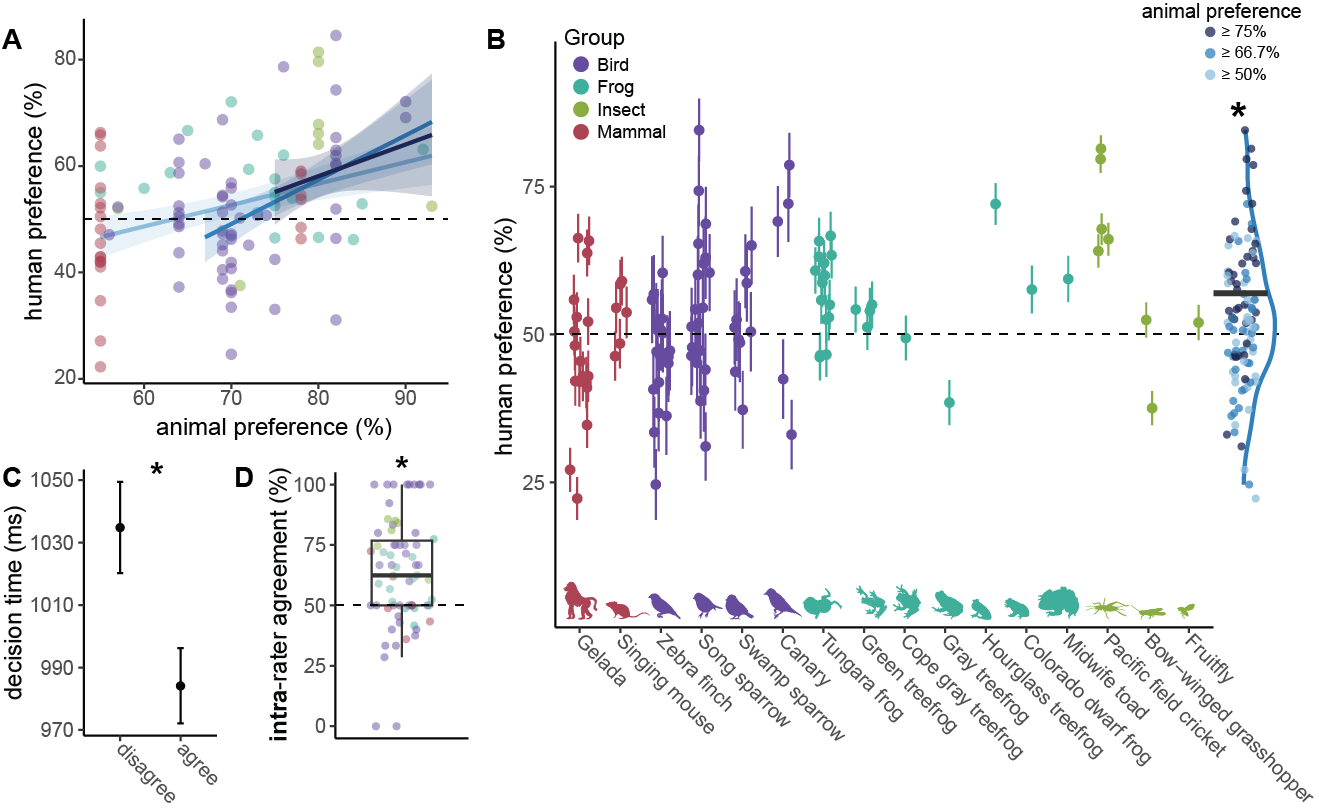
\includegraphics[width=1\linewidth]{../viz/fig1-annotated} 

}

\caption{\textbf{Fig. 1. Humans share acoustic preferences with other animals.} (\textbf{A}) The scatterplot shows the correlation between the strength of the animal's preference for the more-attractive sound in a stimulus pair ($x$-axis) and the percent of humans that preferred the more-attractive sound ($y$-axis). Each dot represents a stimulus pair. Trendlines show simple linear correlations (shading for standard error) when analyzing all stimuli (light blue); stimuli with at least a 2:1 animal preference (medium blue); or stimuli with at least a 3:1 animal preference (dark blue). (\textbf{B}) Humans chose the more-attractive sound above chance. In the main plot, the dots each depict the percent of humans that preferred the more-attractive sound from a given species; the vertical lines represent 95\% confidence intervals; and the horizontal dotted line represents chance (50\%). To the right, each dot represents the mean level of human preferences for a stimulus pair, with color indicating the strength of preference in animals. The solid blue line represents a kernel density estimation and horizontal bar denotes the mean across stimulus pairs with at least a 2:1 preference in animals. (\textbf{C}) Decision-making time was significantly shorter for trials when the participant selected the more-attractive stimulus; the dots depict the mean and the error bars depict 95\% confidence intervals, collapsing across all trials (back-transformed from z-scores for visualization). (\textbf{D}) When participants heard the same stimulus pair more than once, their preferences were maintained, on average. Each dot depicts the mean intra-rater agreement for a stimulus pair, and the boxplot depicts the median, interquartile range, and 1.5xIQR. Across all panels, the colors correspond to large phylogenetic group. $^{\ast}p < 0.05$}\label{fig:fig1}
\end{figure}

\clearpage

Second, agreement between human and animal preferences was higher when
the animals' preferences were more robust. When animals exhibited
moderately strong preferences (at least 2:1 odds, or 67\% preference;
see Methods), humans were significantly more likely than chance to
choose the more-attractive sound (GLMM: mean 56.4\% agreement, 95\% CI:
55.8\%-57.0\%; \emph{z} = 2.3, \emph{p} = 0.02; Fig. 1B). This effect
was slightly weaker when including all stimuli (i.e., including those
with subtle animal preferences; 54.0\% agreement: \emph{z} = 1.9,
\emph{p} = 0.05), and stronger with a more stringent cutoff (at least
3:1 odds: 59.5\% agreement; \emph{z} = 3.4, \emph{p} \textless{} 0.01).
All subsequent analyses use the 2:1 animal preference dataset by
default. Moreover, we found no significant differences in agreement
across the large clades of animals present in the study (birds, mammals,
frogs, or insects; \(\chi^{2}_{3}\) = 3.3, \emph{p} = 0.35).

Third, shared preferences across humans and animals were supported by
two additional measures. Humans answered 51 ms faster, on average, when
choosing the more-attractive sound than the less-attractive one (LMM:
\(\chi^{2}_{1}\) = 32.0, \emph{p} \textless{} 0.01; Fig. 1C). Their
responses were also internally reliable: in a subset of trials, we
played participants the same stimulus pair twice and found their
preference was maintained across both presentations at a rate higher
than chance (63\% were the same choice, on average;
\emph{t}\textsubscript{69} = 5.0, \emph{p} \textless{} 0.01; Fig. 1D).

We next tested the degree to which specific properties of animal sounds
are predictive of human preferences. The stimuli studied here derived
from three classes of experiments, each originally designed to test
whether a specific characteristic was predictive of preferences in
animals. In planned analyses, we asked whether humans similarly
expressed such preferences.

In the first class of experiments, researchers experimentally
manipulated the sounds of animals (Table S1). For example, in three
pairs of frog calls (\emph{38}, \emph{44}) researchers measured frogs'
preferences for frequency-manipulated calls. Our human participants
agreed with the frogs (preferring lower frequency calls; GLMM: \emph{z}
= 3.9, \emph{p} \textless{} 0.01). Similarly, both humans and animals
preferred sounds with acoustic adornments, such as ``trills'',
``clicks'', and ``chucks'' (\emph{z} = 4.0, \emph{p} \textless{} 0.01).
There were no significant effects of agreement for stimuli distinguished
primarily by rate or amplitude modulation (Fig. 2A).

In the second class of experiments, researchers studied animals across
experimental conditions (e.g., varied social contexts) and tested
preferences for the sounds they produced. Surprisingly, humans disagreed
with animals for stimuli that varied in the developmental experience of
the signaler (\emph{z} = -2.5, \emph{p} = 0.01). Specifically, humans
prefer zebra finch songs from males reared without a tutor (``isolate
songs'') over songs from birds that learned their song. We found no
effect of agreement for songs produced in different social contexts or
songs produced with or without a nerve cut (Fig. 2A).

In the third class of experiments, researchers recorded the natural
variation in sounds across individuals, and tested animals' preferences
for them. Humans shared a preference for sounds that had less
evolutionary novelty; both humans and crickets preferred ancestral
``chirps'' over novel ``purrs'' (\emph{z} = 7.3, \emph{p} \textless{}
0.01; Fig. 2A). We also observed a non-significant trend toward
agreement for general individual differences in acoustic structure
(which may signal benefits to the receiver; \emph{z} = 1.7, \emph{p} =
0.08; Fig. 2A).

In exploratory analyses, we also asked whether any single acoustic
feature could predict which stimulus was more attractive to humans
and/or other animals across all stimuli. Consistent with the idea that
preferences arise from complex interactions of multiple cues
(\emph{52}), we did not find that a single acoustic feature predicted
the behavior of both humans and animals. Animals were more likely to
prefer the stimulus with greater brightness, higher spectral centroid,
or shorter duration (Fig. 2B; Table S3), whereas humans were more likely
to prefer the stimulus with lower pitch (Figs. 2B, S3; Table S3).

\begin{figure}

{\centering 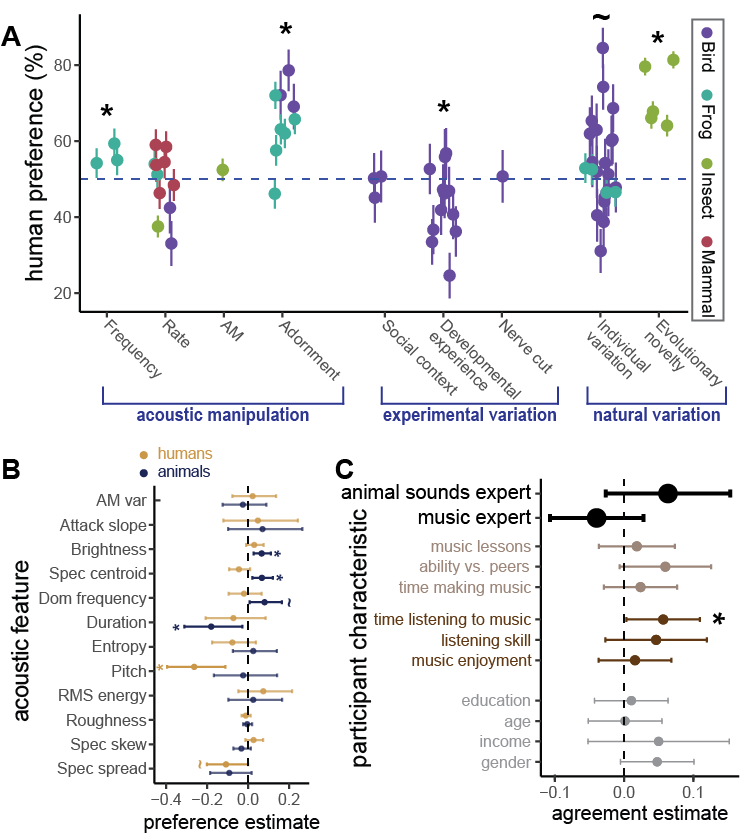
\includegraphics[width=0.7\linewidth]{../viz/fig2-annotated} 

}

\caption{\textbf{Fig. 2. Influence of acoustic traits and participant characteristics on human-animal agreement.} (\textbf{A}) In some cases, variation within stimulus pairs predicted human preferences. There were three categories of variation: acoustic manipulations; experimental variation, where the animals producing the sounds differed on the basis of a manipulation; or natural variation, where the sounds varied without experimental input. Dots denote the mean human preference for the more-attractive sound in each stimulus pair and the vertical lines denote 95\% confidence intervals. (\textbf{B}) Dots denote model estimates (\textit{z}-scores) and horizontal lines denote 95\% confidence intervals for each acoustic feature on human (orange) or animal (blue) preferences. (\textbf{C}) Dots denote estimates from models asking whether a given participant characteristic predicted human agreement with other animals, and the horizontal lines denote 95\% confidence intervals (values binarized for visualization). The two large black dots denote planned analyses and smaller dots indicate exploratory analyses relating to music production (light brown), perception (dark brown), or demographics (grey). $^{\ast}p < 0.05$, $^{\sim}p < 0.10$}\label{fig:figure 2}
\end{figure}

Last, we tested whether characteristics of the participants were
predictive of their agreement with animals. We predicted that prior
experience with animal sounds and musical expertise would predict human
preferences given that experience can shape auditory perception and
preferences (\emph{53}--\emph{56}).

Neither prediction was supported. Humans with experience identifying
animals by their sounds, such as birders (``animal experts'';
\(n = 373\), \textasciitilde9\% of participants), and expert musicians
(\(n = 730\), \textasciitilde19\% of participants) exhibited similar
degrees of agreement as non-experts (GLMMs: animal experts:
\(\chi^{2}_{1}\) = 1.9, \emph{p} = 0.17; music experts: \(\chi^{2}_{1}\)
= 1.3, \emph{p} = 0.25; Fig. 2C). The only significant predictor of
agreement was time listening to music, with those reporting more time
listening to music per day agreeing with animals more (\(\chi^{2}_{1}\)
= 8.5, \emph{p} \textless{} 0.01; Figs. 2C, S1; Table S3).

In exploratory analyses, we asked whether demographic variables (e.g.,
age, gender) predict preference; gender is of particular interest given
that preferences in male animals can be at least as strong as those in
females (\emph{57}, \emph{58}). While no demographic variable predicted
human preference (Fig. 2C; Table S3), one result was intriguing:
analysis of the full dataset (i.e., including the stimuli with weak
animal preferences), revealed a small, statistically significant effect
of participant gender, where male participants agreed with animals more
than female participants. But this result was internally inconsistent
(see Methods), and did not hold when limiting the stimulus set to pairs
with clear preferences in animals. We therefore suggest caution with
interpretation. Finally, human agreement with animals remained
significantly above chance (\emph{z} = 2.3, \emph{p} = 0.02), even when
adjusting the main analysis for demographic variables (gender,
education, age, and income) or time spent listening to music.

\subsection{Discussion}\label{discussion}

We report shared acoustic preferences between humans and other animals,
generalizing across insects, frogs, birds, and non-human mammals. The
strength of preferences for the more-attractive sound was correlated
across humans and animals; humans were more likely than chance to prefer
the more-attractive sound; and humans answered more quickly when
selecting the more-attractive sound.

These results are consistent with general form-function relationships in
acoustic signals across species (\emph{59}--\emph{65}). For example,
sound ``roughness'' is observed in alarm and distress calls and is
perceived as aversive across numerous species (\emph{52},
\emph{66}--\emph{72}). Humans appear to be sensitive to this and other
form-function relationships in other species (\emph{73}--\emph{76}).
Moreover, some animals are sensitive to distress calls from other
species and many animals respond to heterospecific alarm calls
(\emph{77}, \emph{78}). While most studies have focused on sounds used
in aggressive, aversive, or submissive contexts, our results suggest
that cross-species form-function relationships may similarly be used for
preference. Such relationships may underlie the perception of
attractiveness in our own communicative vocalizations, including speech
and music (\emph{52}, \emph{79}--\emph{81}).

There is little evidence about specific features that robustly predict
preferred sounds (\emph{52}, \emph{66}, \emph{80}), consistent with our
finding that no single acoustic feature predicted both human and animal
preferences across all stimuli. Relatively ambiguous measures of sound
(such as ``complexity'') are often proposed to explain preferences
(\emph{82}--\emph{86}). For example, flycatchers and starlings prefer
individuals with more complex (larger) repertoires (\emph{83},
\emph{84}). Humans similarly prefer more complex birdsongs (\emph{87}),
but these measures are difficult to generalize across varied species
(\emph{88}, \emph{89}).

We did find that humans (but not animals) generally preferred the
stimulus with lower pitch (\emph{90}), which may relate to
human-specific pitch perception (\emph{91}). Overall, there were few
similarities across animals and humans in the acoustic characteristics
that served as cues to attractiveness --- despite their shared overall
preferences. Humans' and animals' attractiveness inferences likely
result from multiple, interacting cues, perhaps reflecting cross-species
differences in auditory processing (\emph{22}, \emph{91}, \emph{92}).

Whereas we did not find an effect of experience with animal sounds
{[}cf. (\emph{55}, \emph{93}){]} or music production expertise on
alignment with animal preferences, we did find that higher levels of
music listening experience predicted whether humans agreed with animals.
Music training is known to be associated with advantages in auditory
processing ability (review: \emph{94}), and at least one study shows an
association between auditory discrimination abilities and music
listening time (\emph{95}). Perhaps sustained music listening leads to
increased attention, or better auditory discrimination ability, which
translated to higher concordance with animals {[}whose vocalizations can
share features with music; e.g., (\emph{96}, \emph{97}){]}.

We note that preferences in animals are often subtle, context-dependent,
and can vary across individuals and populations (\emph{98}). This may
account for the high degree of variation in the strength and direction
of human preferences observed across stimuli, and the relatively subtle
main effect of agreement between humans and other animals. The overall
pattern of convergent evidence from multiple analysis approaches,
combined with the increasing robustness when limiting the sample to
stimulus pairs for which animals themselves show stronger preferences,
suggests a robust main effect.

In sum, these results confirm that a single species can harbor similar
preferences to a taxonomically broad range of species. While Darwin's
original idea of shared preferences alluded to the visual coloration of
birds, our findings suggest a more expansive shared ``taste for the
beautiful'' (\emph{23}, \emph{24}), motivating work across many species
and in other modalities (\emph{99}). Finally, these results remind us
that much of the beauty we find in nature was intended for receivers
other than ourselves.

\section{End notes}\label{end-notes}

\subsection{Acknowledgments}\label{acknowledgments}

We thank Elizabeth Adkins-Regan, Jaime Bosch, Katherine Buchanan, Bruce
Byers, Morgan Gustison, Albertine Leitão, Stefan Leitner, Stephen
Nowicki, Bret Pasch, Susan Peters, Michael Reichert, Michael Ritchie,
Ryan Taylor, Robin Tinghitella, Michelle Tomaszycki, Eric-Marie Vallet,
and the Macaulay Library for generously providing acoustic stimuli; Jan
Simson, Isaac Kinley, and Sophia MacNeil for help with code and data
management; and Mila Bertolo, Lidya Yurdum, and the members of the Music
Lab for feedback on the design of the experiment and on the manuscript.

\subsection{Funding}\label{funding}

Smithsonian Institution Postdoctoral Fellowship (LSJ)\\
Fonds de recherche du Québec -- Nature et technologies PR-299652 (SCW,
JTS)\\
US National Institutes of Health DP5OD024566 (SAM)\\
Royal Society of New Zealand Te Apārangi RDF-UOA2103 (SAM)

\subsection{Author contributions}\label{author-contributions}

Conceptualization: LSJ, SCW, JTS, MJR, SAM\\
Methodology: LSJ, JTS, CBH, SAM\\
Data curation: LSJ, CBH, SAM\\
Investigation: LSJ\\
Visualization: LSJ\\
Software: LSJ, CBH\\
Funding acquisition: LSJ, SCW, JTS, SAM\\
Project administration: SAM\\
Supervision: SCW, JTS, MJR, SAM\\
Writing -- original draft: LSJ, SCW, JTS, CBH, MJR, SAM\\
Writing -- review \& editing: LSJ, SCW, JTS, CBH, MJR, SAM

\subsection{Competing interests}\label{competing-interests}

The authors declare that they have no competing interests.

\subsection{Data and materials
availability}\label{data-and-materials-availability}

Data, code, materials, and a reproducible manuscript are available at
\url{https://github.com/themusiclab/animal-sounds}.

\subsection{Supplementary Materials}\label{supplementary-materials}

Materials and Methods\\
Supplementary Text\\
Tables S1 to S3\\
Figures S1 to S3\\
References 100-105

\subsection{References}\label{references}

\footnotesize

\phantomsection\label{refs}
\begin{CSLReferences}{0}{0}
\bibitem[\citeproctext]{ref-bradbury_principles_2011}
\CSLLeftMargin{1. }%
\CSLRightInline{J. W. Bradbury, S. L. Vehrencamp, \emph{Principles of
Animal Communication} (Sinauer Associates, Sunderland, MA, 2011).}

\bibitem[\citeproctext]{ref-andersson_sexual_1994}
\CSLLeftMargin{2. }%
\CSLRightInline{M. Andersson,
\emph{\href{https://www.ncbi.nlm.nih.gov/pubmed/21256434}{Sexual
Selection}} (Princeton University Press, 1994).}

\bibitem[\citeproctext]{ref-coughlan_importance_2020}
\CSLLeftMargin{3. }%
\CSLRightInline{J. M. Coughlan, D. R. Matute,
\href{https://doi.org/10.1098/rstb.2019.0533}{The importance of
intrinsic postzygotic barriers throughout the speciation process}.
\emph{Philosophical Transactions of the Royal Society B: Biological
Sciences} \textbf{375}, 20190533 (2020).}

\bibitem[\citeproctext]{ref-mayr_animal_1963}
\CSLLeftMargin{4. }%
\CSLRightInline{E. Mayr, \emph{Animal Species and Evolution} (Harvard
University Press, 1963).}

\bibitem[\citeproctext]{ref-west-eberhard_sexual_1979}
\CSLLeftMargin{5. }%
\CSLRightInline{M. J. West-Eberhard,
\href{http://www.jstor.org/stable/986582}{Sexual selection, social
competition, and evolution}. \emph{Proceedings of the American
Philosophical Society} \textbf{123}, 222--234 (1979).}

\bibitem[\citeproctext]{ref-guilford_receiver_1993}
\CSLLeftMargin{6. }%
\CSLRightInline{T. Guilford, M. S. Dawkins,
\href{https://doi.org/10.1016/0166-2236(93)90068-W}{Receiver psychology
and the design of animal signals}. \emph{Trends in Neurosciences}
\textbf{16}, 430--436 (1993).}

\bibitem[\citeproctext]{ref-endler_sensory_1998}
\CSLLeftMargin{7. }%
\CSLRightInline{J. Endler, A. Basolo,
\href{https://doi.org/10.1016/S0169-5347(98)01471-2}{Sensory ecology,
receiver biases and sexual selection}. \emph{Trends in Ecology \&
Evolution} \textbf{13}, 415--420 (1998).}

\bibitem[\citeproctext]{ref-ryan_sexual_1998}
\CSLLeftMargin{8. }%
\CSLRightInline{M. J. Ryan,
\href{https://doi.org/10.1126/science.281.5385.1999}{Sexual selection,
receiver biases, and the evolution of sex differences}. \emph{Science}
\textbf{281}, 1999--2003 (1998).}

\bibitem[\citeproctext]{ref-rodd_possible_2002}
\CSLLeftMargin{9. }%
\CSLRightInline{F. H. Rodd, K. A. Hughes, G. F. Grether, C. T. Baril,
\href{https://doi.org/10.1098/rspb.2001.1891}{A possible non-sexual
origin of mate preference: Are male guppies mimicking fruit?}
\emph{Proceedings of the Royal Society of London. Series B: Biological
Sciences} \textbf{269}, 475--481 (2002).}

\bibitem[\citeproctext]{ref-smith_receiver_2004}
\CSLLeftMargin{10. }%
\CSLRightInline{C. Smith, I. Barber, R. J. Wootton, L. Chittka,
\href{https://doi.org/10.1098/rspb.2004.2690}{A receiver bias in the
origin of three--spined stickleback mate choice}. \emph{Proceedings of
the Royal Society of London. Series B: Biological Sciences}
\textbf{271}, 949--955 (2004).}

\bibitem[\citeproctext]{ref-ryan_perceptual_2013}
\CSLLeftMargin{11. }%
\CSLRightInline{M. J. Ryan, M. E. Cummings,
\href{https://doi.org/10.1146/annurev-ecolsys-110512-135901}{Perceptual
biases and mate choice}. \emph{Annual Review of Ecology, Evolution, and
Systematics} \textbf{44}, 437--459 (2013).}

\bibitem[\citeproctext]{ref-renoult_processing_2019}
\CSLLeftMargin{12. }%
\CSLRightInline{J. P. Renoult, T. C. Mendelson,
\href{https://doi.org/10.1098/rspb.2019.0165}{Processing bias: Extending
sensory drive to include efficacy and efficiency in information
processing}. \emph{Proceedings of the Royal Society B: Biological
Sciences} \textbf{286}, 20190165 (2019).}

\bibitem[\citeproctext]{ref-hulse_sexual_2020}
\CSLLeftMargin{13. }%
\CSLRightInline{S. V. Hulse, J. P. Renoult, T. C. Mendelson,
\href{https://www.ncbi.nlm.nih.gov/pubmed/32444815}{Sexual signaling
pattern correlates with habitat pattern in visually ornamented fishes}.
\emph{Nature Communications} \textbf{11} (2020).}

\bibitem[\citeproctext]{ref-rosenthal_sexual_2022}
\CSLLeftMargin{14. }%
\CSLRightInline{G. G. Rosenthal, M. J. Ryan,
\href{https://doi.org/10.1126/science.abi6308}{Sexual selection and the
ascent of women: {Mate} choice research since {Darwin}}. \emph{Science}
\textbf{375}, eabi6308 (2022).}

\bibitem[\citeproctext]{ref-downer-bartholomew_female_2022}
\CSLLeftMargin{15. }%
\CSLRightInline{B. M. B. Downer-Bartholomew, F. H. Rodd,
\href{https://doi.org/10.1093/beheco/arab131}{Female preference for
color-enhanced males: A test of the sensory bias model in medaka, a drab
fish}. \emph{Behavioral Ecology} \textbf{33}, 252--262 (2022).}

\bibitem[\citeproctext]{ref-hamilton_heritable_1982}
\CSLLeftMargin{16. }%
\CSLRightInline{W. D. Hamilton, M. Zuk,
\href{https://doi.org/10.1126/science.7123238}{Heritable true fitness
and bright birds: {A} role for parasites?} \emph{Science} \textbf{218},
384--387 (1982).}

\bibitem[\citeproctext]{ref-hill_plumage_1991}
\CSLLeftMargin{17. }%
\CSLRightInline{G. E. Hill,
\href{https://doi.org/10.1038/350337a0}{Plumage coloration is a sexually
selected indicator of male quality}. \emph{Nature} \textbf{350},
337--339 (1991).}

\bibitem[\citeproctext]{ref-johnstone_sexual_1995}
\CSLLeftMargin{18. }%
\CSLRightInline{R. A. Johnstone,
\href{https://doi.org/10.1111/j.1469-185X.1995.tb01439.x}{Sexual
selection, honest advertisement and the handicap principle: {Reviewing}
the evidence}. \emph{Biological Reviews} \textbf{70}, 1--65 (1995).}

\bibitem[\citeproctext]{ref-balenger_testing_2014}
\CSLLeftMargin{19. }%
\CSLRightInline{S. L. Balenger, M. Zuk,
\href{https://doi.org/10.1093/icb/icu059}{Testing the {Hamilton}-{Zuk}
{Hypothesis}: {Past}, present, and future}. \emph{Integrative and
Comparative Biology} \textbf{54}, 601--613 (2014).}

\bibitem[\citeproctext]{ref-dougherty_meta-analysis_2021}
\CSLLeftMargin{20. }%
\CSLRightInline{L. R. Dougherty,
\href{https://doi.org/10.1038/s41559-021-01409-z}{Meta-analysis reveals
that animal sexual signalling behaviour is honest and resource based}.
\emph{Nature Ecology \& Evolution} \textbf{5}, 688--699 (2021).}

\bibitem[\citeproctext]{ref-rosenthal_mate_2017}
\CSLLeftMargin{21. }%
\CSLRightInline{G. G. Rosenthal, \emph{Mate Choice: The Evolution of
Sexual Decision Making from Microbes to Humans} (Princeton University
Press, Princeton, NJ, 2017).}

\bibitem[\citeproctext]{ref-fay_evolution_2000}
\CSLLeftMargin{22. }%
\CSLRightInline{R. R. Fay, A. N. Popper,
\href{https://doi.org/10.1016/S0378-5955(00)00168-4}{Evolution of
hearing in vertebrates: The inner ears and processing}. \emph{Hearing
Research} \textbf{149}, 1--10 (2000).}

\bibitem[\citeproctext]{ref-darwin_descent_1871}
\CSLLeftMargin{23. }%
\CSLRightInline{C. Darwin, \emph{The Descent of Man and Selection in
Relation to Sex} (Murray, London, 1871).}

\bibitem[\citeproctext]{ref-ryan_taste_2018}
\CSLLeftMargin{24. }%
\CSLRightInline{M. J. Ryan, \emph{A Taste for the Beautiful: {The}
Evolution of Attraction} (Princeton University Press, Princeton, NJ,
2018).}

\bibitem[\citeproctext]{ref-wells_vocal_1984}
\CSLLeftMargin{25. }%
\CSLRightInline{K. D. Wells, J. J. Schwartz,
\href{https://doi.org/10.1016/S0003-3472(84)80277-8}{Vocal communication
in a neotropical treefrog, \emph{{Hyla} ebraccata}: {Advertisement}
calls}. \emph{Animal Behaviour} \textbf{32}, 405--420 (1984).}

\bibitem[\citeproctext]{ref-ryan_tungara_1985}
\CSLLeftMargin{26. }%
\CSLRightInline{M. J. Ryan, \emph{The Túngara Frog - a Study in Sexual
Selection and Communication} (University of Chicago Press, 1985).}

\bibitem[\citeproctext]{ref-ryan_sexual_1993}
\CSLLeftMargin{27. }%
\CSLRightInline{M. J. Ryan, A. S. Rand,
\href{https://doi.org/10.1098/rstb.1993.0057}{Sexual selection and
signal evolution: The ghost of biases past}. \emph{Philosophical
Transactions of the Royal Society of London. Series B: Biological
Sciences} \textbf{340}, 187--195 (1993).}

\bibitem[\citeproctext]{ref-ryan_sexual_2003}
\CSLLeftMargin{28. }%
\CSLRightInline{M. J. Ryan, A. S. Rand,
\href{https://doi.org/10.1111/j.0014-3820.2003.tb01503.x}{Sexual
selection in female perceptual space: {How} female túngara frogs
perceive and respond to complex population variation in acoustic mating
signals}. \emph{Evolution} \textbf{57}, 2608--2618 (2003).}

\bibitem[\citeproctext]{ref-marquez_female_1995}
\CSLLeftMargin{29. }%
\CSLRightInline{R. Márquez,
\href{https://doi.org/10.1163/156853995X00342}{Female choice in the
midwife toads (\emph{{Alytes} obstetricans} and \emph{{A}.
Cisternasii})}. \emph{Behaviour} \textbf{132}, 151--161 (1995).}

\bibitem[\citeproctext]{ref-vallet_female_1995}
\CSLLeftMargin{30. }%
\CSLRightInline{E. Vallet, M. Kreutzer,
\href{https://doi.org/10.1016/0003-3472(95)90082-9}{Female canaries are
sexually responsive to special song phrases}. \emph{Animal Behaviour}
\textbf{49}, 1603--1610 (1995).}

\bibitem[\citeproctext]{ref-vallet_two-note_1998}
\CSLLeftMargin{31. }%
\CSLRightInline{E. Vallet, I. Beme, M. Kreutzer,
\href{https://doi.org/10.1006/anbe.1997.0631}{Two-note syllables in
canary songs elicit high levels of sexual display}. \emph{Animal
Behaviour} \textbf{55}, 291--297 (1998).}

\bibitem[\citeproctext]{ref-ritchie_drosophila_1999}
\CSLLeftMargin{32. }%
\CSLRightInline{M. G. Ritchie, E. J. Halsey, J. M. Gleason,
\href{https://doi.org/10.1006/anbe.1999.1167}{\emph{Drosophila} song as
a species-specific mating signal and the behavioural importance of
{Kyriacou} \& {Hall} cycles in \emph{{D}. Melanogaster} song}.
\emph{Animal Behaviour} \textbf{58}, 649--657 (1999).}

\bibitem[\citeproctext]{ref-leitner_female_2002}
\CSLLeftMargin{33. }%
\CSLRightInline{S. Leitner, C. K. Catchpole,
\href{https://doi.org/10.1002/neu.10085}{Female canaries that respond
and discriminate more between male songs of different quality have a
larger song control nucleus ({HVC}) in the brain}. \emph{Journal of
Neurobiology} \textbf{52}, 294--301 (2002).}

\bibitem[\citeproctext]{ref-nowicki_quality_2002}
\CSLLeftMargin{34. }%
\CSLRightInline{S. Nowicki, W. A. Searcy, S. Peters,
\href{https://doi.org/10.1098/rspb.2002.2124}{Quality of song learning
affects female response to male bird song}. \emph{Proceedings of the
Royal Society of London. Series B: Biological Sciences} \textbf{269},
1949--1954 (2002).}

\bibitem[\citeproctext]{ref-lauay_female_2004}
\CSLLeftMargin{35. }%
\CSLRightInline{C. Lauay, N. M. Gerlach, E. Adkins-Regan, T. J. DeVoogd,
\href{https://doi.org/10.1016/j.anbehav.2003.12.025}{Female zebra
finches require early song exposure to prefer high-quality song as
adults}. \emph{Animal Behaviour} \textbf{68}, 1249--1255 (2004).}

\bibitem[\citeproctext]{ref-tomaszycki_experimental_2005}
\CSLLeftMargin{36. }%
\CSLRightInline{M. L. Tomaszycki, E. Adkins-Regan,
\href{https://doi.org/10.1016/j.anbehav.2005.01.010}{Experimental
alteration of male song quality and output affects female mate choice
and pair bond formation in zebra finches}. \emph{Animal Behaviour}
\textbf{70}, 785--794 (2005).}

\bibitem[\citeproctext]{ref-leitner_immediate_2005}
\CSLLeftMargin{37. }%
\CSLRightInline{S. Leitner, C. Voigt, R. Metzdorf, C. K. Catchpole,
\href{https://doi.org/10.1002/neu.20135}{Immediate early gene ({ZENK},
{Arc}) expression in the auditory forebrain of female canaries varies in
response to male song quality}. \emph{Journal of Neurobiology}
\textbf{64}, 275--284 (2005).}

\bibitem[\citeproctext]{ref-marquez_intensity_2008}
\CSLLeftMargin{38. }%
\CSLRightInline{R. Márquez, J. Bosch, X. Eekhout,
\href{https://doi.org/10.1016/j.anbehav.2007.05.003}{Intensity of female
preference quantified through playback setpoints: Call frequency versus
call rate in midwife toads}. \emph{Animal Behaviour} \textbf{75},
159--166 (2008).}

\bibitem[\citeproctext]{ref-searcy_female_2010}
\CSLLeftMargin{39. }%
\CSLRightInline{W. A. Searcy, S. Peters, S. Kipper, S. Nowicki,
\href{https://doi.org/10.1007/s00265-010-0949-5}{Female response to song
reflects male developmental history in swamp sparrows}. \emph{Behavioral
Ecology and Sociobiology} \textbf{64}, 1343--1349 (2010).}

\bibitem[\citeproctext]{ref-pasch_androgen-dependent_2011}
\CSLLeftMargin{40. }%
\CSLRightInline{B. Pasch, A. S. George, P. Campbell, S. M. Phelps,
\href{https://doi.org/10.1016/j.anbehav.2011.04.018}{Androgen-dependent
male vocal performance influences female preference in {Neotropical}
singing mice}. \emph{Animal Behaviour} \textbf{82}, 177--183 (2011).}

\bibitem[\citeproctext]{ref-akre_signal_2011}
\CSLLeftMargin{41. }%
\CSLRightInline{K. L. Akre, H. E. Farris, A. M. Lea, R. A. Page, M. J.
Ryan, \href{https://doi.org/10.1126/science.1205623}{Signal perception
in frogs and bats and the evolution of mating signals}. \emph{Science}
\textbf{333}, 751--752 (2011).}

\bibitem[\citeproctext]{ref-reichert_noise_2015}
\CSLLeftMargin{42. }%
\CSLRightInline{M. S. Reichert, B. Ronacher,
\href{https://doi.org/10.1111/evo.12592}{Noise affects the shape of
female preference functions for acoustic signals: {Female} preferences
in noise}. \emph{Evolution} \textbf{69}, 381--394 (2015).}

\bibitem[\citeproctext]{ref-reichert_modality_2015}
\CSLLeftMargin{43. }%
\CSLRightInline{M. S. Reichert, G. Höbel,
\href{https://doi.org/10.1111/evo.12750}{Modality interactions alter the
shape of acoustic mate preference functions in gray treefrogs}.
\emph{Evolution} \textbf{69}, 2384--2398 (2015).}

\bibitem[\citeproctext]{ref-laird_multimodal_2016}
\CSLLeftMargin{44. }%
\CSLRightInline{K. L. Laird, P. Clements, K. L. Hunter, R. C. Taylor,
\href{https://doi.org/10.1007/s00265-016-2160-9}{Multimodal signaling
improves mating success in the green tree frog (\emph{{Hyla} cinerea}),
but may not help small males}. \emph{Behavioral Ecology and
Sociobiology} \textbf{70}, 1517--1525 (2016).}

\bibitem[\citeproctext]{ref-gustison_vocal_2016}
\CSLLeftMargin{45. }%
\CSLRightInline{M. L. Gustison, T. J. Bergman,
\href{https://doi.org/10.1038/srep19680}{Vocal complexity influences
female responses to gelada male calls}. \emph{Scientific Reports}
\textbf{6}, 19680 (2016).}

\bibitem[\citeproctext]{ref-chen_courtship_2017}
\CSLLeftMargin{46. }%
\CSLRightInline{Y. Chen, O. Clark, S. C. Woolley,
\href{https://doi.org/10.1098/rspb.2017.0054}{Courtship song preferences
in female zebra finches are shaped by developmental auditory
experience}. \emph{Proceedings of the Royal Society B: Biological
Sciences} \textbf{284}, 20170054 (2017).}

\bibitem[\citeproctext]{ref-tinghitella_purring_2018}
\CSLLeftMargin{47. }%
\CSLRightInline{R. M. Tinghitella, E. D. Broder, G. A. Gurule-Small, C.
J. Hallagan, J. D. Wilson, \href{https://doi.org/10.1086/700116}{Purring
crickets: {The} evolution of a novel sexual signal}. \emph{The American
Naturalist} \textbf{192}, 773--782 (2018).}

\bibitem[\citeproctext]{ref-tinghitella_responses_2021}
\CSLLeftMargin{48. }%
\CSLRightInline{R. M. Tinghitella, E. D. Broder, J. H. Gallagher, A. W.
Wikle, D. M. Zonana,
\href{https://doi.org/10.1038/s41467-021-20971-5}{Responses of intended
and unintended receivers to a novel sexual signal suggest clandestine
communication}. \emph{Nature Communications} \textbf{12}, 797 (2021).}

\bibitem[\citeproctext]{ref-ryan_nineteen_2019}
\CSLLeftMargin{49. }%
\CSLRightInline{M. J. Ryan, K. L. Akre, A. T. Baugh, X. E. Bernal, A. M.
Lea, C. Leslie, M. B. Still, D. C. Wylie, A. S. Rand,
\href{https://doi.org/10.1086/704103}{Nineteen years of consistently
positive and strong female mate preferences despite individual
variation}. \emph{American Naturalist} \textbf{194}, 125--134 (2019).}

\bibitem[\citeproctext]{ref-barr_dopamine_2021}
\CSLLeftMargin{50. }%
\CSLRightInline{H. J. Barr, E. M. Wall, S. C. Woolley,
\href{https://doi.org/10.1016/j.cub.2021.08.005}{Dopamine in the
songbird auditory cortex shapes auditory preference}. \emph{Curr Biol},
1--13 (2021).}

\bibitem[\citeproctext]{ref-long_how_2023}
\CSLLeftMargin{51. }%
\CSLRightInline{B. Long, J. Simson, A. Buxó-Lugo, D. G. Watson, S. A.
Mehr, \href{https://doi.org/10.1038/d41586-023-00065-6}{How games can
make behavioural science better}. \emph{Nature} \textbf{613}, 433--436
(2023).}

\bibitem[\citeproctext]{ref-mcdermott_auditory_2012}
\CSLLeftMargin{52. }%
\CSLRightInline{J. H. McDermott,
{``\href{https://doi.org/10.1016/B978-0-12-381431-9.00020-6}{Auditory
preferences and aesthetics}''} in \emph{Neuroscience of {Preference} and
{Choice}} (Elsevier, 2012), pp. 227--256.}

\bibitem[\citeproctext]{ref-liu_language_2023}
\CSLLeftMargin{53. }%
\CSLRightInline{J. Liu, C. B. Hilton, E. Bergelson, S. A. Mehr,
\href{https://doi.org/10.1016/j.cub.2023.03.067}{Language experience
predicts music processing in a half-million speakers of fifty-four
languages}. \emph{Current Biology} \textbf{33}, 1916--1925.e4 (2023).}

\bibitem[\citeproctext]{ref-krumhansl_cascading_2013}
\CSLLeftMargin{54. }%
\CSLRightInline{C. L. Krumhansl, J. A. Zupnick,
\href{https://doi.org/10.1177/0956797613486486}{Cascading reminiscence
bumps in popular music}. \emph{Psychological Science} \textbf{24},
2057--2068 (2013).}

\bibitem[\citeproctext]{ref-rosenstein_birdsong_2024}
\CSLLeftMargin{55. }%
\CSLRightInline{R. Rosenstein, M. L. Goldblatt,
\href{https://doi.org/10.1163/15685306-bja10206}{Birdsong complexity and
preference: {The} role of birdwatching expertise}. \emph{Society \&
Animals}, 1--19 (2024).}

\bibitem[\citeproctext]{ref-mcpherson-mcnato_preferences_2026}
\CSLLeftMargin{56. }%
\CSLRightInline{M. J. McPherson-McNato, E. A. Undurraga, S. E. Dolan, A.
Durango, B. J. Medina, R. A. Godoy, J. H. McDermott,
\href{https://doi.org/10.1016/j.cognition.2025.106333}{Preferences for
consonance are evident in {Indigenous} {Amazonians} with higher, but not
lower, levels of global integration}. \emph{Cognition} \textbf{267},
106333 (2026).}

\bibitem[\citeproctext]{ref-mendelson_preference_2018}
\CSLLeftMargin{57. }%
\CSLRightInline{T. C. Mendelson, J. M. Gumm, M. D. Martin, P. J.
Ciccotto, \href{https://doi.org/10.1111/evo.13406}{Preference for
conspecifics evolves earlier in males than females in a sexually
dimorphic radiation of fishes}. \emph{Evolution} \textbf{72}, 337--347
(2018).}

\bibitem[\citeproctext]{ref-hejjabrichard_comparative_2024}
\CSLLeftMargin{58. }%
\CSLRightInline{Y. Héjja‐Brichard, J. P. Renoult, T. C. Mendelson,
\href{https://doi.org/10.1002/ece3.11498}{Comparative analysis reveals
assortative mate preferences in darters independent of sympatry and
sex}. \emph{Ecology and Evolution} \textbf{14}, e11498 (2024).}

\bibitem[\citeproctext]{ref-morton_occurrence_1977}
\CSLLeftMargin{59. }%
\CSLRightInline{E. S. Morton, \href{https://doi.org/10.1086/283219}{On
the occurrence and significance of motivation-structural rules in some
bird and mammal sounds}. \emph{The American Naturalist} \textbf{111},
855--869 (1977).}

\bibitem[\citeproctext]{ref-arnal_human_2015}
\CSLLeftMargin{60. }%
\CSLRightInline{L. H. Arnal, A. Flinker, A. Kleinschmidt, A.-L. Giraud,
D. Poeppel, \href{https://doi.org/10.1016/j.cub.2015.06.043}{Human
screams occupy a privileged niche in the communication soundscape}.
\emph{Current Biology} \textbf{25}, 2051--2056 (2015).}

\bibitem[\citeproctext]{ref-blasi_soundmeaning_2016}
\CSLLeftMargin{61. }%
\CSLRightInline{D. E. Blasi, S. Wichmann, H. Hammarström, P. F. Stadler,
M. H. Christiansen,
\href{https://doi.org/10.1073/pnas.1605782113}{Sound--meaning
association biases evidenced across thousands of languages}.
\emph{Proceedings of the National Academy of Sciences} \textbf{113},
10818--10823 (2016).}

\bibitem[\citeproctext]{ref-mehr_form_2018}
\CSLLeftMargin{62. }%
\CSLRightInline{S. A. Mehr, M. Singh, H. York, L. Glowacki, M. M.
Krasnow, \href{https://doi.org/10.1016/j.cub.2017.12.042}{Form and
function in human song}. \emph{Current Biology} \textbf{28}, 356--368.e5
(2018).}

\bibitem[\citeproctext]{ref-mehr_universality_2019}
\CSLLeftMargin{63. }%
\CSLRightInline{S. A. Mehr, M. Singh, D. Knox, D. M. Ketter, D.
Pickens-Jones, S. Atwood, C. Lucas, N. Jacoby, A. A. Egner, E. J.
Hopkins, R. M. Howard, J. K. Hartshorne, M. V. Jennings, J. Simson, C.
M. Bainbridge, S. Pinker, T. J. O'Donnell, M. M. Krasnow, L. Glowacki,
\href{https://doi.org/10.1126/science.aax0868}{Universality and
diversity in human song}. \emph{Science} \textbf{366}, eaax0868 (2019).}

\bibitem[\citeproctext]{ref-hilton_acoustic_2022}
\CSLLeftMargin{64. }%
\CSLRightInline{C. B. Hilton, C. J. Moser, M. Bertolo, H. Lee-Rubin, D.
Amir, C. M. Bainbridge, J. Simson, D. Knox, L. Glowacki, E. Alemu, A.
Galbarczyk, G. Jasienska, C. T. Ross, M. B. Neff, A. Martin, L. K.
Cirelli, S. E. Trehub, J. Song, M. Kim, A. Schachner, T. A. Vardy, Q. D.
Atkinson, A. Salenius, J. Andelin, J. Antfolk, P. Madhivanan, A.
Siddaiah, C. D. Placek, G. D. Salali, S. Keestra, M. Singh, S. A.
Collins, J. Q. Patton, C. Scaff, J. Stieglitz, S. C. Cutipa, C. Moya, R.
R. Sagar, M. Anyawire, A. Mabulla, B. M. Wood, M. M. Krasnow, S. A.
Mehr, \href{https://doi.org/10.1038/s41562-022-01410-x}{Acoustic
regularities in infant-directed speech and song across cultures}.
\emph{Nature Human Behaviour} \textbf{6}, 1545--1556 (2022).}

\bibitem[\citeproctext]{ref-singh_universality_2023}
\CSLLeftMargin{65. }%
\CSLRightInline{M. Singh, S. A. Mehr,
\href{https://doi.org/10.1038/s44159-023-00182-z}{Universality,
domain-specificity and development of psychological responses to music}.
\emph{Nature Reviews Psychology} \textbf{2}, 333--346 (2023).}

\bibitem[\citeproctext]{ref-kumar_mapping_2008}
\CSLLeftMargin{66. }%
\CSLRightInline{S. Kumar, H. M. Forster, P. Bailey, T. D. Griffiths,
\href{https://doi.org/10.1121/1.3006380}{Mapping unpleasantness of
sounds to their auditory representation}. \emph{The Journal of the
Acoustical Society of America} \textbf{124}, 3810--3817 (2008).}

\bibitem[\citeproctext]{ref-gotz_aversiveness_2010}
\CSLLeftMargin{67. }%
\CSLRightInline{T. Götz, V. M. Janik,
\href{https://doi.org/10.1242/jeb.035535}{Aversiveness of sounds in
phocid seals: Psycho-physiological factors, learning processes and
motivation}. \emph{Journal of Experimental Biology} \textbf{213},
1536--1548 (2010).}

\bibitem[\citeproctext]{ref-soltis_measuring_2011}
\CSLLeftMargin{68. }%
\CSLRightInline{J. Soltis, T. E. Blowers, A. Savage,
\href{https://doi.org/10.1121/1.3531798}{Measuring positive and negative
affect in the voiced sounds of {African} elephants (\emph{{Loxodonta}
africana})}. \emph{The Journal of the Acoustical Society of America}
\textbf{129}, 1059--1066 (2011).}

\bibitem[\citeproctext]{ref-hechavarria_bats_2020}
\CSLLeftMargin{69. }%
\CSLRightInline{J. C. Hechavarría, M. Jerome Beetz, F. García-Rosales,
M. Kössl, \href{https://doi.org/10.1038/s41598-020-64323-7}{Bats
distress vocalizations carry fast amplitude modulations that could
represent an acoustic correlate of roughness}. \emph{Scientific Reports}
\textbf{10}, 7332 (2020).}

\bibitem[\citeproctext]{ref-marx_occurrences_2021}
\CSLLeftMargin{70. }%
\CSLRightInline{A. Marx, R. Lenkei, P. Pérez Fraga, V. Bakos, E.
Kubinyi, T. Faragó,
\href{https://doi.org/10.1038/s41598-021-83614-1}{Occurrences of
non-linear phenomena and vocal harshness in dog whines as indicators of
stress and ageing}. \emph{Scientific Reports} \textbf{11}, 4468 (2021).}

\bibitem[\citeproctext]{ref-anikin_harsh_2021}
\CSLLeftMargin{71. }%
\CSLRightInline{A. Anikin, K. Pisanski, M. Massenet, D. Reby,
\href{https://doi.org/10.1098/rspb.2021.0872}{Harsh is large: Nonlinear
vocal phenomena lower voice pitch and exaggerate body size}.
\emph{Proceedings of the Royal Society B: Biological Sciences}
\textbf{288}, 20210872 (2021).}

\bibitem[\citeproctext]{ref-di_stefano_roughness_2022}
\CSLLeftMargin{72. }%
\CSLRightInline{N. Di Stefano, C. Spence,
\href{https://doi.org/10.3758/s13414-022-02550-y}{Roughness perception:
{A} multisensory/crossmodal perspective}. \emph{Attention, Perception,
\& Psychophysics} \textbf{84}, 2087--2114 (2022).}

\bibitem[\citeproctext]{ref-kelly_adult_2017}
\CSLLeftMargin{73. }%
\CSLRightInline{T. Kelly, D. Reby, F. Levréro, S. Keenan, E. Gustafsson,
A. Koutseff, N. Mathevon,
\href{https://doi.org/10.1093/biolinnean/blw016}{Adult human perception
of distress in the cries of bonobo, chimpanzee, and human infants}.
\emph{Biological Journal of the Linnean Society} \textbf{120}, 919--930
(2017).}

\bibitem[\citeproctext]{ref-filippi_humans_2017}
\CSLLeftMargin{74. }%
\CSLRightInline{P. Filippi, J. V. Congdon, J. Hoang, D. L. Bowling, S.
A. Reber, A. Pašukonis, M. Hoeschele, S. Ocklenburg, B. de Boer, C. B.
Sturdy, A. Newen, O. Güntürkün,
\href{https://doi.org/10.1098/rspb.2017.0990}{Humans recognize emotional
arousal in vocalizations across all classes of terrestrial vertebrates:
Evidence for acoustic universals}. \emph{Proceedings of the Royal
Society B: Biological Sciences} \textbf{284}, 20170990 (2017).}

\bibitem[\citeproctext]{ref-kamiloglu_human_2020}
\CSLLeftMargin{75. }%
\CSLRightInline{R. G. Kamiloğlu, K. E. Slocombe, D. B. M. Haun, D. A.
Sauter, \href{https://doi.org/10.1098/rspb.2020.1148}{Human listeners'
perception of behavioural context and core affect dimensions in
chimpanzee vocalizations}. \emph{Proceedings of the Royal Society B:
Biological Sciences} \textbf{287}, 20201148 (2020).}

\bibitem[\citeproctext]{ref-terrade_nonlinear_2025}
\CSLLeftMargin{76. }%
\CSLRightInline{A. Terrade, M. Massenet, L. Pernel, N. Mathevon, A.
Anikin, D. Reby,
\href{https://doi.org/10.1016/j.isci.2025.112600}{Nonlinear phenomena
make animal calls alarming for human listeners}. \emph{iScience}
\textbf{28}, 112600 (2025).}

\bibitem[\citeproctext]{ref-lingle_deer_2014}
\CSLLeftMargin{77. }%
\CSLRightInline{S. Lingle, T. Riede,
\href{https://doi.org/10.1086/677677}{Deer mothers are sensitive to
infant distress vocalizations of diverse mammalian species}. \emph{The
American Naturalist} \textbf{184}, 510--522 (2014).}

\bibitem[\citeproctext]{ref-magrath_eavesdropping_2015}
\CSLLeftMargin{78. }%
\CSLRightInline{R. D. Magrath, T. M. Haff, P. M. Fallow, A. N. Radford,
\href{https://doi.org/10.1111/brv.12122}{Eavesdropping on heterospecific
alarm calls: From mechanisms to consequences}. \emph{Biological Reviews}
\textbf{90}, 560--586 (2015).}

\bibitem[\citeproctext]{ref-feinberg_manipulations_2005}
\CSLLeftMargin{79. }%
\CSLRightInline{D. R. Feinberg, B. C. Jones, A. C. Little, D. M. Burt,
D. I. Perrett,
\href{https://doi.org/10.1016/j.anbehav.2004.06.012}{Manipulations of
fundamental and formant frequencies influence the attractiveness of
human male voices}. \emph{Animal Behaviour} \textbf{69}, 561--568
(2005).}

\bibitem[\citeproctext]{ref-fruhholz_vocal_2018}
\CSLLeftMargin{80. }%
\CSLRightInline{K. Pisanski, D. R. Feinberg,
{``\href{https://doi.org/10.1093/oxfordhb/9780198743187.013.27}{Vocal
{Attractiveness}}''} in \emph{The {Oxford} {Handbook} of {Voice}
{Perception}}, S. Frühholz, P. Belin, Eds. (Oxford University Press,
2018), pp. 606--626.}

\bibitem[\citeproctext]{ref-mehr_toward_2021}
\CSLLeftMargin{81. }%
\CSLRightInline{S. A. Mehr, M. M. Krasnow, G. A. Bryant, E. H. Hagen,
\href{https://doi.org/10.1017/S0140525X21000030}{Toward a productive
evolutionary understanding of music}. \emph{Behavioral and Brain
Sciences} \textbf{44}, e122 (2021).}

\bibitem[\citeproctext]{ref-ryan_female_1980}
\CSLLeftMargin{82. }%
\CSLRightInline{M. J. Ryan,
\href{https://doi.org/10.1126/science.209.4455.523}{Female mate choice
in a neotropical frog}. \emph{Science} \textbf{209}, 523--525 (1980).}

\bibitem[\citeproctext]{ref-lampe_female_1995}
\CSLLeftMargin{83. }%
\CSLRightInline{H. M. Lampe, G. Saetre,
\href{https://doi.org/10.1098/rspb.1995.0191}{Female pied flycatchers
prefer males with larger song repertoires}. \emph{Proceedings of the
Royal Society of London. Series B: Biological Sciences} \textbf{262},
163--167 (1995).}

\bibitem[\citeproctext]{ref-mountjoy_female_1996}
\CSLLeftMargin{84. }%
\CSLRightInline{D. J. Mountjoy, R. E. Lemon,
\href{https://doi.org/10.1007/s002650050218}{Female choice for complex
song in the {European} starling: A field experiment}. \emph{Behavioral
Ecology and Sociobiology} \textbf{38}, 65--71 (1996).}

\bibitem[\citeproctext]{ref-reichert_exploring_2017}
\CSLLeftMargin{85. }%
\CSLRightInline{M. S. Reichert, J. Finck, B. Ronacher,
\href{https://doi.org/10.1111/evo.13202}{Exploring the hidden landscape
of female preferences for complex signals}. \emph{Evolution}
\textbf{71}, 1009--1024 (2017).}

\bibitem[\citeproctext]{ref-choi_increased_2022}
\CSLLeftMargin{86. }%
\CSLRightInline{N. Choi, M. Adams, K. Fowler-Finn, E. Knowlton, M.
Rosenthal, A. Rundus, R. D. Santer, D. Wilgers, E. A. Hebets,
\href{https://doi.org/10.1098/rsbl.2022.0052}{Increased signal
complexity is associated with increased mating success}. \emph{Biology
Letters} \textbf{18}, 20220052 (2022).}

\bibitem[\citeproctext]{ref-da_silva_like_2022}
\CSLLeftMargin{87. }%
\CSLRightInline{O. C. Da Silva, A. M. Melo Santos, N. Schiel, A. Souto,
\href{https://doi.org/10.1080/08927936.2021.1963546}{Like music to our
ears: {The} complexity of bird vocalizations as a key factor of
attractiveness}. \emph{Anthrozoös} \textbf{35}, 91--104 (2022).}

\bibitem[\citeproctext]{ref-patricelli_new_2016}
\CSLLeftMargin{88. }%
\CSLRightInline{G. L. Patricelli, E. A. Hebets,
\href{https://doi.org/10.1016/j.cobeha.2016.09.011}{New dimensions in
animal communication: The case for complexity}. \emph{Current Opinion in
Behavioral Sciences} \textbf{12}, 80--89 (2016).}

\bibitem[\citeproctext]{ref-odom_comparative_2021}
\CSLLeftMargin{89. }%
\CSLRightInline{K. J. Odom, M. Araya-Salas, J. L. Morano, R. A. Ligon,
G. M. Leighton, C. C. Taff, A. H. Dalziell, A. C. Billings, R. R.
Germain, M. Pardo, L. G. de Andrade, D. Hedwig, S. C. Keen, Y. Shiu, R.
A. Charif, M. S. Webster, A. N. Rice,
\href{https://doi.org/10.1111/brv.12695}{Comparative bioacoustics: A
roadmap for quantifying and comparing animal sounds across diverse
taxa}. \emph{Biological Reviews} \textbf{1} (2021).}

\bibitem[\citeproctext]{ref-schwartz_pitch_2024}
\CSLLeftMargin{90. }%
\CSLRightInline{J. W. Schwartz, K. H. Pierson, A. K. Reece,
\href{https://doi.org/10.1037/com0000366}{Pitch affects human
(\emph{{Homo} sapiens}) perception of emotional arousal from diverse
animal calls.} \emph{Journal of Comparative Psychology} \textbf{138},
80--87 (2024).}

\bibitem[\citeproctext]{ref-mehr_core_2025}
\CSLLeftMargin{91. }%
\CSLRightInline{S. A. Mehr,
\href{https://doi.org/10.1016/j.tics.2025.05.013}{Core systems of music
perception}. \emph{Trends in Cognitive Sciences} \textbf{29}, 763--777
(2025).}

\bibitem[\citeproctext]{ref-mcdermott_are_2004}
\CSLLeftMargin{92. }%
\CSLRightInline{J. McDermott, M. Hauser,
\href{https://doi.org/10.1016/j.cognition.2004.04.004}{Are consonant
intervals music to their ears? {Spontaneous} acoustic preferences in a
nonhuman primate}. \emph{Cognition} \textbf{94}, B11--B21 (2004).}

\bibitem[\citeproctext]{ref-chartrand_brain_2007}
\CSLLeftMargin{93. }%
\CSLRightInline{J.-P. Chartrand, S. Filion-Bilodeau, P. Belin,
\href{https://doi.org/10.1097/WNR.0b013e328013cea9}{Brain response to
birdsongs in bird experts}. \emph{NeuroReport} \textbf{18}, 335--340
(2007).}

\bibitem[\citeproctext]{ref-neves_does_2022}
\CSLLeftMargin{94. }%
\CSLRightInline{L. Neves, A. I. Correia, S. L. Castro, D. Martins, C. F.
Lima, \href{https://doi.org/10.1016/j.neubiorev.2022.104777}{Does music
training enhance auditory and linguistic processing? {A} systematic
review and meta-analysis of behavioral and brain evidence}.
\emph{Neuroscience \& Biobehavioral Reviews} \textbf{140}, 104777
(2022).}

\bibitem[\citeproctext]{ref-wesseldijk_does_2020}
\CSLLeftMargin{95. }%
\CSLRightInline{L. W. Wesseldijk, F. Ullén, M. A. Mosing,
\href{https://doi.org/10.1016/j.paid.2020.110001}{Does listening to
music increase your ability to discriminate musical sounds?}
\emph{Personality and Individual Differences} \textbf{161}, 110001
(2020).}

\bibitem[\citeproctext]{ref-roeske_categorical_2020}
\CSLLeftMargin{96. }%
\CSLRightInline{T. C. Roeske, O. Tchernichovski, D. Poeppel, N. Jacoby,
\href{https://doi.org/10.1016/j.cub.2020.06.072}{Categorical rhythms are
shared between songbirds and humans}. \emph{Current Biology}
\textbf{30}, 3544--3555.e6 (2020).}

\bibitem[\citeproctext]{ref-james_pervasive_2024}
\CSLLeftMargin{97. }%
\CSLRightInline{L. S. James, K. Oudyk, E. M. Wall, Y. Chen, W. D.
Pearse, J. T. Sakata, Pervasive patterns in the songs of passerine birds
resemble human music universals and are linked with production and
cognitive mechanisms (2024).
\url{https://doi.org/10.1101/2024.07.15.603339}.}

\bibitem[\citeproctext]{ref-jennions_variation_1997}
\CSLLeftMargin{98. }%
\CSLRightInline{M. D. Jennions, M. Petrie,
\href{https://doi.org/10.1111/j.1469-185X.1997.tb00015.x}{Variation in
mate choice and mating preferences: {A} review of causes and
consequences}. \emph{Biological Reviews} \textbf{72}, 283--327 (1997).}

\bibitem[\citeproctext]{ref-ghirlanda_chickens_2002}
\CSLLeftMargin{99. }%
\CSLRightInline{S. Ghirlanda, L. Jansson, M. Enquist,
\href{https://doi.org/10.1007/s12110-002-1021-6}{Chickens prefer
beautiful humans}. \emph{Human Nature} \textbf{13}, 383--389 (2002).}

\bibitem[\citeproctext]{ref-de_leeuw_jspsych_2023}
\CSLLeftMargin{100. }%
\CSLRightInline{J. R. De Leeuw, R. A. Gilbert, B. Luchterhandt,
\href{https://doi.org/10.21105/joss.05351}{{jsPsych}: {Enabling} an
{open}-{source} {collaborative} {ecosystem} of {behavioral}
{experiments}}. \emph{Journal of Open Source Software} \textbf{8}, 5351
(2023).}

\bibitem[\citeproctext]{ref-peretz_prevalence_2017}
\CSLLeftMargin{101. }%
\CSLRightInline{I. Peretz, D. T. Vuvan,
\href{https://doi.org/10.1038/ejhg.2017.15}{Prevalence of congenital
amusia}. \emph{European Journal of Human Genetics} \textbf{25}, 625--630
(2017).}

\bibitem[\citeproctext]{ref-bertolo_humans_2025}
\CSLLeftMargin{102. }%
\CSLRightInline{M. Bertolo, M. W. Weiss, I. Peretz, J. T. Sakata,
Humans, but not songbirds, produce spontaneously isochronous song
through the lifespan (2025).
\url{https://doi.org/10.1101/2025.06.02.657467}.}

\bibitem[\citeproctext]{ref-lartillot2007matlab}
\CSLLeftMargin{103. }%
\CSLRightInline{O. Lartillot, P. Toiviainen, {``A matlab toolbox for
musical feature extraction from audio''} in \emph{International
Conference on Digital Audio Effects} (Bordeaux, 2007)vol. 237, p. 244.}

\bibitem[\citeproctext]{ref-bates_package_2007}
\CSLLeftMargin{104. }%
\CSLRightInline{D. Bates, M. Maechler, B. Bolker, S. Walker, Package
'lme4'. \emph{R Package} (2007).}

\bibitem[\citeproctext]{ref-fox_hypothesis_2013}
\CSLLeftMargin{105. }%
\CSLRightInline{J. Fox, M. Friendly, S. Weisberg,
\href{https://doi.org/10.32614/RJ-2013-004}{Hypothesis tests for
multivariate linear models using the car {Package}}. \emph{The R
Journal} \textbf{5}, 39 (2013).}

\end{CSLReferences}

\normalsize

\section{Materials and Methods}\label{materials-and-methods}

\subsection{Participants}\label{participants}

Participants were visitors to the citizen-science website
\url{https://themusiclab.org} between 2023-09-06 and 2025-09-15 (Fig.
S1). Participants were recruited through word of mouth, classroom
activities, social media, and targeted newsletters (e.g., Animal
Behavior Society). They were not compensated.

We analyzed data from participants who (i) reported age between 18-90;
(ii) reported wearing headphones and/or ``in a very quiet place''; (iii)
reported no hearing impairment; and (iv) reported fluency in English,
either as their native or second language. These inclusion criteria were
determined before analyzing any data, so could not bias the results in
any direction. All participants gave informed consent under ethics
protocols approved by the Yale University Human Research Protection
Program (protocol 2000033433) and the McGill University Research Ethics
Board (initial approval October 24, 2022; protocol 22-09-042).

\subsection{Stimuli}\label{stimuli}

We obtained audio files used in a variety of published studies, with the
exception of a few stimuli which came from the unpublished collections
of colleagues or a public sound library (Macaulay Library; Table S1). In
general, audio was requested from scientists by the first author
(L.S.J.) based on their studies of conspecific acoustic preferences
(i.e., in research where preferences had been measured in receivers of
the species that produced the sound). In general, we opted not to use
stimuli where the most salient difference between stimuli was in
amplitude or duration. All stimuli were produced by male animals, and
preference studies were conducted with females as the receivers.

For 14 out of 24 sets of stimuli, stimulus pairs were experimentally
manipulated by the researchers. For example, in singing mouse songs,
trill rates were experimentally modified digitally. These techniques are
common in studies of animal preference, which typically seek to control
for precise differences between pairs of sounds. Because we aimed to
study the concordance between human preferences and animal preferences,
and because animal preferences had been measured using these stimuli in
previous work, we treated manipulated stimuli interchangeably with
unaltered ones. Table S1 indicates which stimuli were fully naturalistic
recordings and which were altered for the preference experiment(s) they
were gathered from.

We normalized the stimuli by peak amplitude using Audacity software
(\url{https://www.audacityteam.org}). In one case (singing mouse) the
stimuli were near the upper frequency threshold for sound detection in
humans; to ensure our participants could hear them clearly, we
pitch-shifted them down two octaves, also in Audacity.

All audio files can be accessed at
\url{http://github.com/themusiclab/animal-sounds}.

\subsection{Experimental design}\label{experimental-design}

Participants listened to 16 pairs of stimuli (4 drawn at random with
replacement from each of the four categories of frogs, birds, mammals,
and insects), presented in random order. Because stimuli were selected
at random with replacement, some participants received the same pair of
stimuli more than once, providing an opportunity to measure intra-rater
reliability.

On each trial, the first sound of a pair played after a half-second of
silence. To maintain visual interest, as the sound played, an animal
silhouette appeared on left side of the screen with a slight animated
movement. The silhouette then disappeared, and after one second of
silence, the second sound played, in conjunction with a second animal
silhouette on the right side of the screen. The left stimulus always
appeared first and the right stimulus always appeared second, but the
order of presentation within pairs was randomized, such that the
more-attractive sound preceded the less-attractive sound roughly as
often as the reverse. Throughout, large text on the screen indicated the
prompt ``Which call do you \textbf{like} more?''. After one-tenth of a
second of silence, both silhouettes reappeared and participants could
respond. The means of response depended on device type: on desktop or
laptop computers, the silhouettes were labelled with an ``F'' or ``J''
underneath (the left and right silhouette, respectively), and
participants used their keyboard to enter their response; while on
mobile devices (including tablets), participants tapped the left or
right side of the screen. Participants on desktop or laptop computers
could also enter responses by using a mouse click or touchscreen tap,
but we encouraged them to use the keyboard to improve the validity of
response time data.

Before and after the 16 trials described above, participants completed
self-report questions on a variety of topics (see Demographic analyses,
below).

Following the experiment, as an incentive for participation, we
displayed a customized graphic indicating which of the four animal
categories their responses agreed most with, along with descriptive
information about the sounds of that animal category. This facilitated
the sharing of results, spurring recruitment of more participants, a
common strategy in gamified citizen science (\emph{51}). Note that we
did not indicate whether participants correctly identified the
more-attractive sound during the experiment, precluding any learning
effects during the experiment.

The experiment was implemented using the jsPsych ecosystem for
behavioral experiments {[}\url{https://jspsych.org}; (\emph{100}){]} and
hosted using the WorldWideLab backend (\url{https://worldwidelab.org}).
Readers can try the experiment at
\url{https://themusiclab.org/quizzes/havoc}. Code for the experiment is
available at \url{https://github.com/themusiclab/animal-sounds}.

\subsection{Demographic analyses}\label{demographic-analyses}

We collected demographic data on participants to evaluate factors that
could shape auditory preferences for non-human animal signals. Not all
participants answered all demographic items; as such, we report the
proportion of responses for each item as opposed to raw \emph{N}s.

To identify ``experts'' in animal sounds, we asked ``\emph{Do you have a
hobby or job where you identify animals by their sounds? For example
birdwatching, herping, zookeeping, etc.}'' Participants responding
``\emph{Yes}'' were considered to be experts.

To identify ``experts'' in music, we asked ``\emph{Think of your skill
at making music (using a musical instrument or singing). How would you
rate your own skill?}''. Participants that answered ``\emph{I'm an
expert}'' or ``\emph{I have a lot of skill}'' were considered to be
experts, in contrast to those that answered ``\emph{I have no skill at
all}'', ``\emph{I have some skill}'', or ``\emph{I'm a novice}'' (i.e.,
this item was recoded as a binary category).

In addition to these data, which were used for planned analyses (see
Main Text), we studied 10 additional variables in exploratory analyses
of how experience and other variables impact participant responses.
These included:

\begin{itemize}
\tightlist
\item
  gender (male, female or other)
\item
  age (in years)
\item
  education (8 ordered responses from ``\emph{Some elementary/middle
  school}'' to ``\emph{Completed graduate school}'')
\item
  income (9 ordered responses from ``\emph{Under \$10,000'' to ''Over
  \$150,000}''), asked only of those reporting being located in the
  United States
\item
  daily time spent making music (9 ordered responses from ``\emph{no
  time}'' to ``\emph{\textgreater{} 4 hours}'')
\item
  daily time spent listening to music (9 ordered responses from
  ``\emph{no time}'' to ``\emph{\textgreater{} 4 hours}'')
\item
  music lessons experience (binary variable)
\item
  for participants who had completed music lessons, music skill in
  childhood, in relation to peers (5 ordered responses from ``\emph{They
  were a lot better than me}'' to ``\emph{I was a lot better than
  them}'')
\item
  music listening skill, with the text ``\emph{How good do you think
  your music listening skills are? (things like remembering melodies,
  hearing out of tune notes, or hearing a beat that is out of sync with
  the music)}'' with responses on a sliding scale from ``\emph{I'm much
  worse than other people}'' to ``\emph{I'm much better than other
  people}'' with scale points unlabeled
\item
  degree of music enjoyment, with the text ``\emph{In general, how much
  do you enjoy music?}'' with a comparable sliding scale to (9), but
  anchors labeled ``\emph{I don't enjoy music very much}'' and ``\emph{I
  enjoy music very much}''
\end{itemize}

While many participants completed additional self-report items as part
of their visit to \url{https://themusiclab.org}, we did not analyze them
in this paper.

In a few cases, the variables required trimming or transformation. We
detail these decisions below:

\begin{itemize}
\tightlist
\item
  Values for age were z-transformed.\\
\item
  For the two sliding scales (music listening skill and degree of music
  enjoyment), we observed unusual response distributions with multiple
  peaks in responses, suggesting irregular response patterns. The
  default answer for both sliders was 500 (out of 1000); for both items,
  we omitted responses of exactly 500 (i.e., the participant did not
  move the slider: 587 out of 4165 participants and 229 out of 4164,
  respectively). We proceeded with two transformations:

  \begin{itemize}
  \tightlist
  \item
    For music listening skill we binarized the data using the midpoint
    of the scale, classifying only participants who moved the slider to
    the right as ``skilled'' relative to the other participants.\\
  \item
    For degree of music enjoyment, we noted that about half the
    participants moved the slider all the way to the right anchor
    (1000), so rather than binarizing based on the midpoint of the
    scale, we classified those right-anchored participants as
    ``enjoyers'' relative to all other participants.
  \end{itemize}
\item
  While we used all data as described here in the statistical models
  (see below and in Main Text), to facilitate visual comparison of the
  effect sizes across each variable, in the figures, we binarized the
  numeric variables based on the mean value of the variable across
  participants.\\
\item
  Finally, when including demographic covariates within our main model
  testing whether participants agreed with animals more than chance, we
  z-transformed the data.
\end{itemize}

We note that all trimming and transformation strategies for these
exploratory analyses were determined without knowledge of the results.

All demographic variables were self-reported, thus will have some error
based on biases in responses from participants. However, previous
studies using self-disclosure of pitch perception or music expertise
found strong correlations between the self-reported measures and
performance on music perception tests (\emph{101}, \emph{102}),
suggesting that such items reliably track some aspects of cognition.

\subsection{Acoustic analyses}\label{acoustic-analyses}

We measured 12 acoustic features using MATLAB. Three were calculated
based on the waveform (dominant frequency, duration, and the amplitude
modulation variance) and the remaining 9 were measured using
\texttt{MIRtoolbox} (\emph{103}), a package commonly used for music
information retrieval: pitch (``best'' prediction of the pitch),
spectral centroid, brightness, roughness, Shannon entropy, attack slope,
RMS energy (global energy), spectral skewness, and spectral spread.
These metrics provide broad summaries of the sounds and do not describe
acoustic patterning in detail.

Because the absolute level of each acoustic feature varies widely across
species (e.g., pitch is far higher for \emph{all} birds than for
\emph{all} frogs), we could not simply regress human preferences on
acoustic characteristics. Instead, we first computed difference scores
for each feature within each stimulus pair (i.e., subtracting the value
for the less-attractive sound from the value for the more-attractive
sound). These difference scores highlight what acoustic features are
meaningful in distinguishing attractiveness across stimulus pairs,
independently of the absolute level of specific acoustic features.

We studied the acoustic difference scores in relation to the estimated
preferences of humans or animals. Specifically, we tested whether the
more-attractive stimulus in each pair systematically varied as a
function of acoustic features, relative to the less-attractive stimulus
(e.g., for the feature of pitch, testing whether humans consistently
selected the sound with lower pitch more often than expected by chance).
Finally, we asked whether differences in acoustic features could predict
whether humans chose the more-attractive stimulus (e.g., for the feature
of pitch, testing whether larger differences in pitch between the two
stimuli led to higher degrees of human-animal agreement).

In some cases, acoustic features could not be calculated (i.e., the
function produced an NA value); we excluded those stimuli from analysis.
This affected 5 stimulus pairs from the analysis of pitch (canary songs,
likely due to the synthesized nature of the songs), 4 pairs from the
analysis of spectral centroid (cricket and grasshopper songs, likely due
to the broadband nature of their ``clicks''), and 5 pairs from the
analysis of attack slope (cricket and sparrow songs). Further, we
assessed the distributions of difference scores for normality, and
removed outliers: we omitted 3 pairs from the analysis of dominant
frequency, 3 pairs from the analysis of spectral centroid, and 2 pairs
from the analysis of roughness. Visual exclusion of outliers was done
prior to conducting any statistical models and blind to the identity
(e.g., species) of the outliers.

\subsection{Estimated strength of animal
preference}\label{estimated-strength-of-animal-preference}

For each stimulus pair, we used previous literature to generate an
estimate of the strength of acoustic preference in the species that
originally produced the sound. Given the heterogeneity of methods used
in the studies from which we gathered the sounds, this required
combining several approaches.

When studies had presented animals with binary choices between pairs of
sounds, we computed the percent of animals choosing the preferred
stimulus as the strength of preference (n.b., this measure is akin to
the measure of human preference in our experiment, which was also a
binary choice). When studies had used other behavioral measures, such as
a count of the number of actions elicited by the sounds, we compared the
magnitude of the behavioral result across stimulus types and calculated
the percent of responses for the more-attractive sounds. When studies
had used multiple behavioral responses with the same species and
stimuli, we prioritized those that were most directly interpretable,
e.g., those where animals' movement toward or time spent near a speaker
indicated their choice. We did so with the goal of enabling clear
comparisons across studies and taxa.

For example, in a study of single phonotaxis tests in crickets, 78.3\%
of the crickets tested approached the preferred songs while only 19.1\%
of the crickets approached the unpreferred songs (\emph{48}). Thus, out
of all responses, 80\% were for the preferred stimulus, indicating the
strength of preference {[}78.3/(78.3 + 19.1) = 80.4{]}. In a more
complex example, a study of swamp sparrow females found a mean of 6.9
copulation solicitation displays in response to more-attractive songs
and only 3.9 displays in response to less-attractive songs (\emph{39}).
Thus, we estimated the strength of preference at 64\% {[}6.9/(6.9 + 3.9)
= 63.9{]}.

While we typically used the exact values reported in published papers,
when these values were not available, we used the PlotDigitizer tool
(\url{https://plotdigitizer.com}) to estimate values visually from
figures.

The strength of animal preference was variable (range: 55\% -- 93\%
preference), representing approximately 5:4 to 15:1 odds. We used this
variation to test whether the strength of animal preference predicted
the strength of human preference (see below). However, we also conducted
analyses limited to relatively strong animal preferences. Specifically,
we limited those analyses to stimuli with at least a 2:1 odds preference
(\(\geq66.67\%\); e.g., for every one individual that picked the
less-preferred stimulus, two individuals picked the preferred stimulus)
or at least a 3:1 odds preference (\(\geq75\%\)).

\subsection{Statistical approaches}\label{statistical-approaches}

To test whether participants selected the animal-preferred stimulus more
than expected by chance, we used an intercept-only generalized linear
mixed effects model (GLMM) with a binary response variable (1 = agreed
with animals, i.e., chose the more-attractive sound, from the animal's
perspective; 0 = disagree) and a binomial link function, using
\texttt{lme4} (\emph{104}). We included Stimulus Pair ID, Species ID,
and Participant ID as random effects, to license generalization across
the sounds, species, and participants studied. These models all estimate
the overall degree of agreement and test that estimate against a chance
level of 0.5.

We used the same analytic approach for other key measures of interest,
such as analyzing decision-making time, comparing the strength of
preference between humans and animals, and assessing the influence of
participant-level covariates on the main effects. Some data
transformation was required for decision-making time analyses (i.e.,
square-root and z-transformed to improve model assumptions, limited to
responses \textless{} 5 sec). To measure intra-rater reliability, we
coded whether a participant selected the same (1) or different (0) sound
across two repeated presentations, averaged these values for each
stimulus pair, and tested this value against chance level of 50\% with
an intercept-only linear model (i.e., a one-sample \emph{t}-test) across
all stimuli.

For the acoustic feature analyses, we asked whether the value of any
acoustic feature predicted whether humans or non-human animals preferred
a stimulus in a pair, using mixed-effects models with an acoustic
feature as the dependent variable, whether the stimulus was preferred
(either by animals or by humans (greater than 50\% human choice) in
separate models) as an independent binary categorical factor, and
Stimulus Pair ID and Species ID as random effects. We also asked whether
the difference in a feature between the two stimuli could predict
agreement between humans and animals, using linear mixed effects models
with the size of the acoustic difference (computed by subtracting the
value for the less-attractive sound from the value for the
more-attractive sound) as the independent variable, average percent
agreement (percent of human choices for the animal's preferred stimulus)
as the dependent variable, and Species ID as a random effect.

Full model specifications are available in the R Markdown manuscript
available at \url{https://github.com/themusiclab/animal-sounds}. We used
the \texttt{car} package for Type II Wald chi-square tests (\emph{105})
for significance testing in the GLMMs and Type III analyses of variance
with Satterthwaite's method for the LMMs. When models failed to
converge, we removed the random effect of species, and found nearly
identical results. For any models with singular fits, the stimulus
random intercept was dropped.

\subsection{Gender effects}\label{gender-effects}

While we limited our primary analyses to stimuli for which animals
exhibited at least moderately strong preferences (2:1 odds, 66.67\%
preference), in preliminary analyses using the entire stimulus dataset,
we found a significant effect of participant gender (male, female, or
other) on their agreement with animals (\(\chi^{2}_{2}\) = 11.0,
\emph{p} \textless{} 0.01). Post-hoc contrasts indicated that male
participants exhibited significantly greater agreement with other
animals than female participants (\emph{p} \textless{} 0.01), and no
pairwise differences with participants with a gender of ``other''
(\emph{p} \textgreater{} 0.61 for both). However, we note that the
preferences of male and female participants were highly and
significantly correlated (\(r^{2}\) = 0.7, \emph{p} \textless{} 0.01),
and as reported in the main text, the effect does not hold in our
analysis limited to at least a 2:1 preference in animals. This indicates
that the gender effect is primarily driven by responses to stimuli with
the most ambiguity in animal preference (i.e., the stimuli where we have
the least confidence in our estimation of the more-attractive stimulus).

Finally, we highlight that, in our primary analyses, all effects hold
when limited to a single gender (significant difference from chance:
male: \emph{z} = 2.4, \emph{p} = 0.02; female: \emph{z} = 2.0, \emph{p}
= 0.04; other: \emph{z} = 2.2, \emph{p} = 0.03; correlation between
animal preference and human preference strength: male: \(\chi^{2}_{1}\)
= 5.5, p = 0.02; female: \(\chi^{2}_{1}\) = 4.3, p = 0.04; other:
\(\chi^{2}_{1}\) = 5.7, p = 0.02). As such, we suggest caution in
interpreting gender effects and encourage future research on this
subject.

\clearpage

\section{Supplementary tables and
figures}\label{supplementary-tables-and-figures}

\footnotesize

\textbf{Table S1. Description of stimuli.} Note. ``N'' refers to the
number of stimulus pairs; ``Altered'' refers to whether the sounds were
experimentally manipulated; ``Same stim'' refers to whether or not we
were able to obtain and use the exact stimuli tested on the animals
themselves, or used other sources; ``CSDs'' refers to copulation
solicitation displays.

\begin{longtable}[]{@{}
  >{\raggedright\arraybackslash}p{(\linewidth - 14\tabcolsep) * \real{0.1216}}
  >{\raggedleft\arraybackslash}p{(\linewidth - 14\tabcolsep) * \real{0.1216}}
  >{\raggedright\arraybackslash}p{(\linewidth - 14\tabcolsep) * \real{0.0946}}
  >{\raggedright\arraybackslash}p{(\linewidth - 14\tabcolsep) * \real{0.1081}}
  >{\raggedright\arraybackslash}p{(\linewidth - 14\tabcolsep) * \real{0.1486}}
  >{\raggedright\arraybackslash}p{(\linewidth - 14\tabcolsep) * \real{0.1216}}
  >{\raggedright\arraybackslash}p{(\linewidth - 14\tabcolsep) * \real{0.1486}}
  >{\raggedright\arraybackslash}p{(\linewidth - 14\tabcolsep) * \real{0.1351}}@{}}
\toprule\noalign{}
\begin{minipage}[b]{\linewidth}\raggedright
Species
\end{minipage} & \begin{minipage}[b]{\linewidth}\raggedleft
N pairs
\end{minipage} & \begin{minipage}[b]{\linewidth}\raggedright
Trait
\end{minipage} & \begin{minipage}[b]{\linewidth}\raggedright
Method
\end{minipage} & \begin{minipage}[b]{\linewidth}\raggedright
Direction
\end{minipage} & \begin{minipage}[b]{\linewidth}\raggedright
Altered
\end{minipage} & \begin{minipage}[b]{\linewidth}\raggedright
Same stim
\end{minipage} & \begin{minipage}[b]{\linewidth}\raggedright
Citation
\end{minipage} \\
\midrule\noalign{}
\endhead
\bottomrule\noalign{}
\endlastfoot
Canary (\emph{Serinus canaria}) & 3 & Adornment & CSDs & & Y & Y &
(\emph{30}, \emph{31}, \emph{33}, \emph{37}) \\
Canary (\emph{Serinus canaria}) & 2 & Rate & CSDs & Faster & Y & Y &
(\emph{30}, \emph{31}, \emph{33}, \emph{37}) \\
Song sparrow (\emph{Melospiza melodia}) & 10 & Individuals & CSDs & & N
& Y & (\emph{34}) \\
Song sparrow (\emph{Melospiza melodia}) & 10 & Individuals & CSDs & & N
& Y & (\emph{34}) \\
Swamp sparrow (\emph{Melospiza georgiana}) & 10 & Development
(nutritional stress) & CSDs & & N & Y & (\emph{39}) \\
Zebra finch (\emph{Taeniopygia castanotis}) & 4 & Social context & Call
backs & & N & Y & (\emph{46}) \\
Zebra finch (\emph{Taeniopygia castanotis}) & 12 & Development (isolate
reared) & Time near speaker & & N & N & (\emph{35}); Adkins-Regan \\
Zebra finch (\emph{Taeniopygia castanotis}) & 2 & Individuals & String
pulls & & N & Y & (\emph{50}) \\
Zebra finch (\emph{Taeniopygia castanotis}) & 1 & Manipulated (nerve
cut) & Time near speaker & & N & Y & (\emph{36}) \\
Colorado dwarf frog (\emph{Engystomops coloradorum}) & 1 & Adornment &
Two speaker phonotaxis & & Y & Y & (\emph{27}) \\
Cope's gray treefrog (\emph{Hyla chrysoscelis}) & 1 & Rate & & Faster &
Y & N & \\
Gray treefrog (\emph{Hyla versicolor}) & 1 & Rate & & Average & Y & Y &
(\emph{43}) \\
Green treefrog (\emph{Hyla cinerea}) & 2 & Frequency & Two speaker
phonotaxis & Lower & Y & Y & (\emph{44}) \\
Green treefrog (\emph{Hyla cinerea}) & 2 & Rate & Two speaker phonotaxis
& Faster & Y & Y & (\emph{44}) \\
Hourglass treefrog (\emph{Dendropsophus ebraccatus}) & 1 & Adornment &
Two speaker phonotaxis & & Y & N & (\emph{25}); from Macaulay \\
Midwife toad (\emph{Alytes obstetricans}) and (\emph{A. cisternasii}) &
1 & Frequency & Two speaker phonotaxis & Lower & Y & Y & (\emph{29},
\emph{38}) \\
Túngara frog (\emph{Engystomops pustulosus}) & 11 & Adornment & Two
speaker phonotaxis & & Y & Y & (\emph{41}, \emph{49}) \\
Túngara frog (\emph{Engystomops pustulosus}) & 4 & Individuals & Two
speaker phonotaxis & & N & Y & (\emph{28}) \\
Bow-winged grasshopper (\emph{Chorthippus biguttulus}) & 1 & Amplitude
modulation & Single speaker phonotaxis & More & Y & Y & (\emph{42}) \\
Bow-winged grasshopper (\emph{Chorthippus biguttulus}) & 1 & Rate &
Single speaker phonotaxis & Faster & Y & Y & (\emph{42}) \\
Fruit fly (\emph{Drosophila melanogaster}) & 1 & Rhythm & Single speaker
phonotaxis & Arrhythmic & Y & Y & (\emph{32}) \\
Pacific field cricket (\emph{Teleogryllus oceanicus}) & 5 & Evolutionary
novelty & Single speaker phonotaxis & Less & N & Y & (\emph{47},
\emph{48}) \\
Gelada (\emph{Theropithecus gelada}) & 18 & Evolutionary novelty & Time
near speaker & More & N & Y & (\emph{45}) \\
Singing mouse (\emph{Scotinomys teguina}) & 6 & Rate & Time near speaker
& Faster & Y & Y & (\emph{40}) \\
\end{longtable}

\normalsize

\textbf{Table S2. Acoustic results.} Note. ``DF'' refers to degrees of
freedom. A ``Diff'' comparison asks whether the difference in a feature
between the stimuli in the pair predicted agreement between humans and
non-human animals; ``Animals'' and ``Humans'' comparisons ask whether
that group demonstrates a directional preference for the feature. ``AM
var'' refers to amplitude modulation variance and ``RMS energy'' refers
to the root-mean-square energy (overall measure of energy in the sound).

\begin{longtable}[]{@{}
  >{\raggedright\arraybackslash}p{(\linewidth - 12\tabcolsep) * \real{0.2568}}
  >{\raggedright\arraybackslash}p{(\linewidth - 12\tabcolsep) * \real{0.1486}}
  >{\raggedleft\arraybackslash}p{(\linewidth - 12\tabcolsep) * \real{0.0811}}
  >{\raggedright\arraybackslash}p{(\linewidth - 12\tabcolsep) * \real{0.0811}}
  >{\raggedright\arraybackslash}p{(\linewidth - 12\tabcolsep) * \real{0.0676}}
  >{\raggedright\arraybackslash}p{(\linewidth - 12\tabcolsep) * \real{0.1486}}
  >{\raggedright\arraybackslash}p{(\linewidth - 12\tabcolsep) * \real{0.2162}}@{}}
\toprule\noalign{}
\begin{minipage}[b]{\linewidth}\raggedright
feature
\end{minipage} & \begin{minipage}[b]{\linewidth}\raggedright
comparison
\end{minipage} & \begin{minipage}[b]{\linewidth}\raggedleft
DFnum
\end{minipage} & \begin{minipage}[b]{\linewidth}\raggedright
DFden
\end{minipage} & \begin{minipage}[b]{\linewidth}\raggedright
F
\end{minipage} & \begin{minipage}[b]{\linewidth}\raggedright
p
\end{minipage} & \begin{minipage}[b]{\linewidth}\raggedright
direction
\end{minipage} \\
\midrule\noalign{}
\endhead
\bottomrule\noalign{}
\endlastfoot
Dominant frequency & Diff & 1 & 61.1 & 0.1 & 0.75 & \\
Dominant frequency & Animals & 1 & 66.0 & 3.5 & 0.07 & \\
Dominant frequency & Humans & 1 & 66.0 & 0.2 & 0.65 & \\
Duration & Diff & 1 & 64.5 & 0.4 & 0.54 & \\
Duration & Animals & 1 & 69.0 & 5.4 & \textbf{0.02} & Prefer longer \\
Duration & Humans & 1 & 69.0 & 0.8 & 0.37 & \\
Pitch & Diff & 1 & 59.3 & 12.2 & \textbf{\textless{} 0.01} & \\
Pitch & Animals & 1 & 64.0 & 0.1 & 0.78 & \\
Pitch & Humans & 1 & 64.0 & 11.4 & \textbf{\textless{} 0.01} & Prefer
lower \\
AM var & Diff & 1 & 66.1 & 0.4 & 0.54 & \\
AM var & Animals & 1 & 127.8 & 0.2 & 0.66 & \\
AM var & Humans & 1 & 127.8 & 0.1 & 0.71 & \\
Spectral centroid & Diff & 1 & 60.9 & 2.8 & 0.10 & \\
Spectral centroid & Animals & 1 & 62.0 & 6.1 & \textbf{0.02} & Prefer
higher \\
Spectral centroid & Humans & 1 & 62.0 & 2.6 & 0.11 & \\
Skew & Diff & 1 & 44.7 & 1.4 & 0.24 & \\
Skew & Animals & 1 & 128.0 & 1.9 & 0.17 & \\
Skew & Humans & 1 & 128.0 & 1.3 & 0.26 & \\
Spread & Diff & 1 & 29.2 & 1.2 & 0.29 & \\
Spread & Animals & 1 & 69.0 & 2.7 & 0.10 & \\
Spread & Humans & 1 & 69.0 & 3.9 & 0.05 & \\
Shannon entropy & Diff & 1 & 31.3 & 1.3 & 0.26 & \\
Shannon entropy & Animals & 1 & 127.8 & 0.2 & 0.67 & \\
Shannon entropy & Humans & 1 & 127.8 & 1.7 & 0.19 & \\
Roughness & Diff & 1 & 65.8 & 0.6 & 0.46 & \\
Roughness & Animals & 1 & 125.0 & 0.1 & 0.72 & \\
Roughness & Humans & 1 & 125.0 & 0.9 & 0.35 & \\
Attack slope & Diff & 1 & 63.0 & 1.2 & 0.28 & \\
Attack slope & Animals & 1 & 64.0 & 0.5 & 0.48 & \\
Attack slope & Humans & 1 & 64.0 & 0.2 & 0.63 & \\
RMS energy & Diff & 1 & 65.3 & 0.2 & 0.67 & \\
RMS energy & Animals & 1 & 128.1 & 0.1 & 0.73 & \\
RMS energy & Humans & 1 & 128.1 & 1.1 & 0.30 & \\
Brightness & Diff & 1 & 54.8 & 0.9 & 0.34 & \\
Brightness & Animals & 1 & 128.0 & 8.3 & \textbf{\textless{} 0.01} &
Prefer brighter \\
Brightness & Humans & 1 & 128.0 & 1.6 & 0.21 & \\
\end{longtable}

\normalsize

\textbf{Table S3. Statistical results for demographics.} Note: The
chi-squared tests are omnibus tests from the GLMMs described under
``Demographic analyses'' in the Methods.

\begin{longtable}[]{@{}llrl@{}}
\toprule\noalign{}
trait & Chisq & DF & p \\
\midrule\noalign{}
\endhead
\bottomrule\noalign{}
\endlastfoot
animal sounds expert & 1.9 & 1 & 0.17 \\
music expert & 1.3 & 1 & 0.25 \\
music lessons & 0.4 & 1 & 0.51 \\
ability wrt peers & 3.1 & 1 & 0.08 \\
time making music & 0.7 & 1 & 0.41 \\
time listening to music & 8.5 & 1 & \textbf{\textless{} 0.01} \\
listening skill & 1.5 & 1 & 0.22 \\
music enjoyment & 0.3 & 1 & 0.56 \\
education & 1.3 & 1 & 0.26 \\
age & 0.7 & 1 & 0.42 \\
income & 1.8 & 1 & 0.18 \\
gender & 3.1 & 2 & 0.21 \\
\end{longtable}

\begin{figure}

{\centering 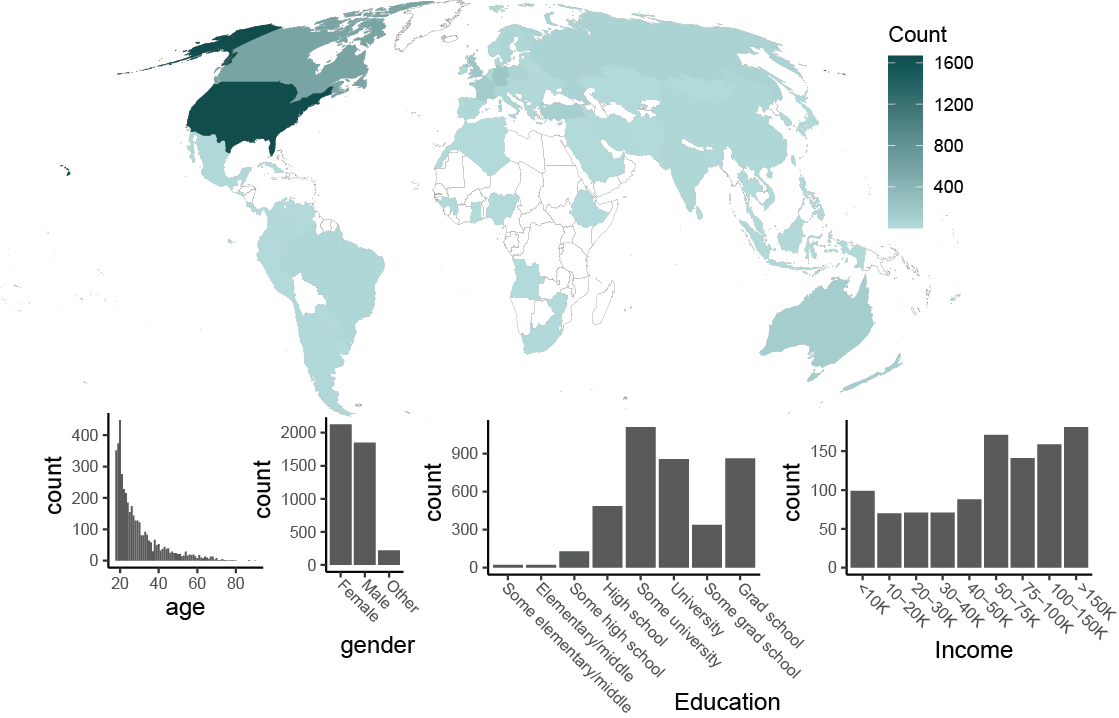
\includegraphics[width=0.9\linewidth]{../viz/FigureS1} 

}

\caption{\textbf{Fig. S1. Participant demographics.} The map depicts the distribution of participants, with darker-shades indicating a larger number of participants who were resident in each country. The bar plots show the distributions of participants' age (in years), gender, education, and income levels of participants.}\label{fig:figure S1}
\end{figure}

\begin{figure}

{\centering 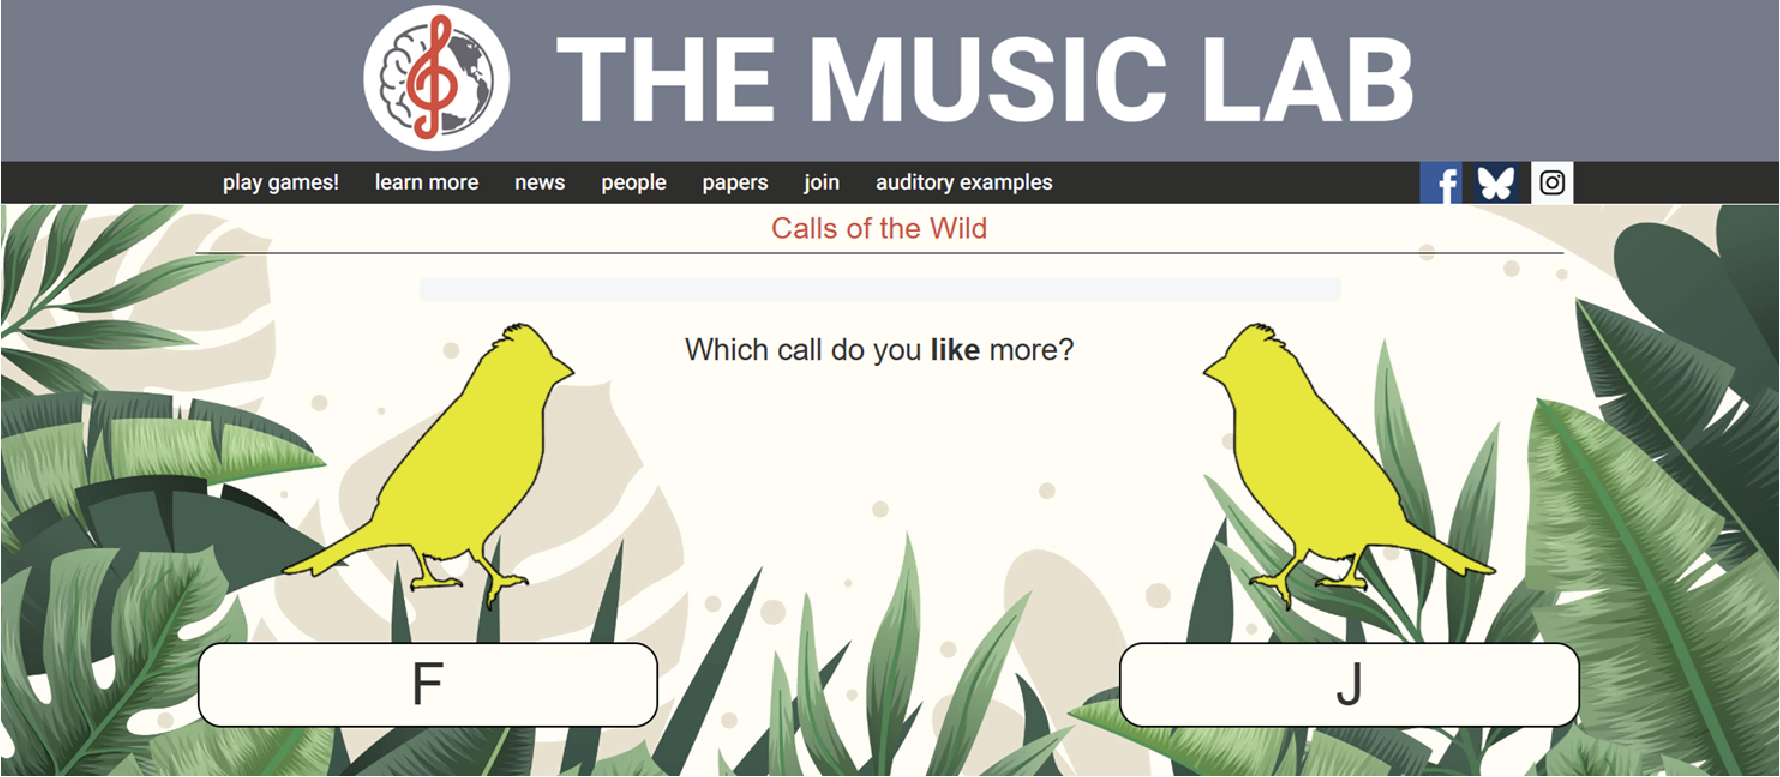
\includegraphics[width=0.9\linewidth]{../viz/FigureS2} 

}

\caption{\textbf{Fig. S2. User interface.} The screenshot shows the experiment's user interface, as appearing for participants who used a desktop or laptop computer. This screen appears after both sounds on a given trial have played and the participant responds by pressing the F or J key on their keyboard (or clicking or tapping one of the two bird silhouettes).}\label{fig:figure S2}
\end{figure}

\begin{figure}

{\centering 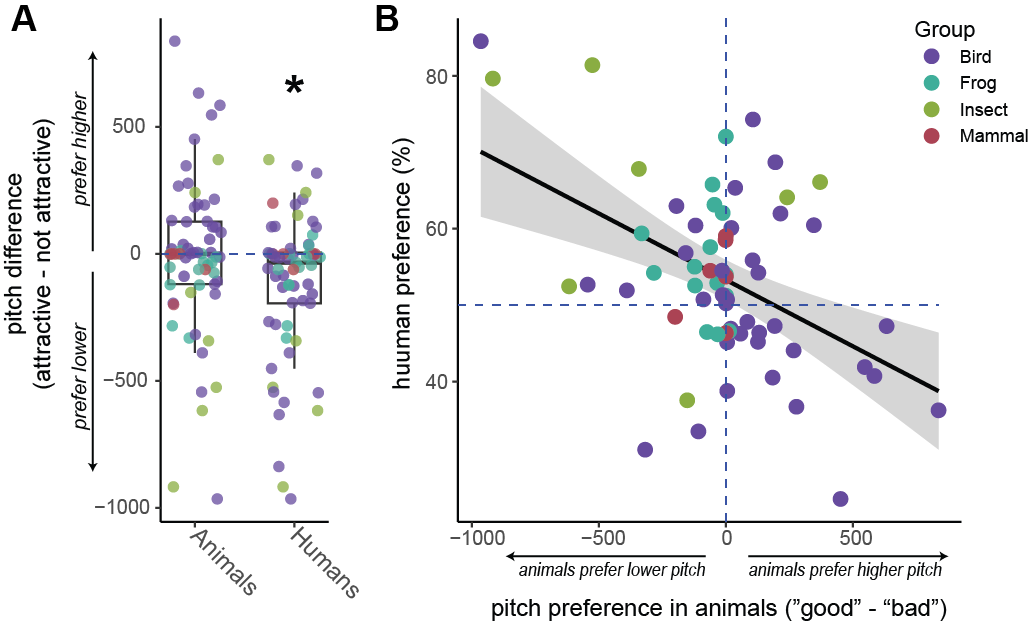
\includegraphics[width=0.9\linewidth]{../viz/FigureS3} 

}

\caption{\textbf{Fig. S3. Influence of pitch on animal and human preferences.} (\textbf{A}) Across all stimulus pairs, humans tended to choose the stimulus with the lower pitch, while there was no consistent preference across the other animals. (\textbf{B}) The difference in pitch within a pair of stimuli was predictive of the degree of human agreement with animals ("human preference"; i.e., humans were more likely to agree with animals when the animal-preferred stimulus was lower in pitch).}\label{fig:figure S3}
\end{figure}

\end{document}
